\section{Preliminaries}
We first introduce some additional notations and describe simplifications that will be used later in the appendix.
\subsection{Definitions}
We sometimes want to iterate over $k$ canonical vectors. We define the following shorthand notation:
\begin{align*}
  \ffor{v_1,\ldots, v_k}{X}{e(X,v_1,\ldots, v_n)}\coloneqq  &\ffor{v_1}{X_1}{X_1 +} \\
  &\hspace{1em}\initf{X_1}{v_2}{X_2}{X_2 + } \\
  &\hspace{2em}\initf{X_2}{v_3}{X_3}{X_3 + } \\
  &\hspace{8em}\ddots \\
  &\hspace{4em}\initf{X_{k-1}}{v_k}{X_k}{ e(X_k,v_1,\ldots, v_k)}.
\end{align*}
To reference $\ell$ different vector variables $X_1,\ldots,X_\ell$ in every iteration and update them in different ways we define:
\begin{multline*}
\ffor{v}{X_1,\ldots, X_\ell}{\left( e_1(X_1,v), e_2(X_2,v), \ldots, e_l(X_\ell,v) \right)} \coloneqq 
\ffor{v}{X}{e_1(X\cdot e_{\mathsf{min}},v)\cdot (e_{\diag}(e_{\ones}(X^T))\cdot e_{\mathsf{min}})^T +\\ e_2(X\cdot e_{\mathsf{min} + 1},v)\cdot (e_{\diag}(e_{\ones}(X^T))\cdot e_{\mathsf{min} + 1})^T + \ldots + e_\ell(X\cdot e_{\mathsf{max}},v)\cdot (e_{\diag}(e_{\ones}(X^T))\cdot e_{\mathsf{max}})^T}
\end{multline*}
We note that for the latter expression to be semantically correct $v$ has to be of type $\gamma\times 1$, 
both $X_i$ and $e_i$ for $ i=1,\ldots,\ell$ have to be of type $\alpha\times 1$, 
and $X$ has to be of type $\alpha\times\beta$, where $\dom(\beta)=\ell$. Here
we use $e_{\diag}(e_{\ones}(X^T))$ to compute the $\beta\times\beta$ identity and ensure the typing of the
$e_{\mathsf{min} + i}$.
% \floris{I believe that $\gamma$ should be $\alpha$? Also, this implies that we cannot loop over more than $\alpha$ different vector variables. Does this cause a problem later on?}
% \thomas{I changed the semantics to be more general, now $v$ can be of any type independently of $X, X_1,...$, and its typing is ensured by the typing of the $e_i$}
When evaluated on an instance $\I$,
$e_{\mathsf{min}}, e_{\mathsf{min} + i}$ evaluate to $b_1^{\dom(\beta)}$ and $b_{1+i}^{\dom(\beta)}$, 
respectively, and we show their defining expressions in section \ref{app:order}.
Similarly for $e_{\mathsf{max}}=b_n^{\dom(\beta)}$.
The combinations of both previous operators results in:
$$
\ffor{v_1,\ldots, v_k}{X_1,\ldots, X_\ell}{\left( e_1(X_1,v_1,\ldots, v_k), e_2(X_2,v_1,\ldots, v_k), \ldots, e_\ell(X_\ell,v_1,\ldots, v_k) \right)} \coloneqq \ffor{v_1,\ldots, v_k}{X}{e'(X,v_1,\ldots, v_k)}
$$
where 
\begin{align}
e'(X,v_1,\ldots,v_k)\coloneqq &e_1(X\cdot e_{\mathsf{min}},v_1,\ldots,v_k)\cdot (e_{\diag}(e_{\ones}(X^T))\cdot e_{\mathsf{min}})^T \\
&+ e_2(X\cdot e_{\mathsf{min} + 1},v_1,\ldots,v_k)\cdot (e_{\diag}(e_{\ones}(X^T))\cdot e_{\mathsf{min} + 1})^T \\
&+ \ldots + e_\ell(X\cdot e_{\mathsf{max}},v_1,\ldots,v_k)\cdot (e_{\diag}(e_{\ones}(X^T))\cdot e_{\mathsf{max}})^T
\end{align}
It is clear that this expression iterates over $k$ canonical vectors and references $\ell$ independent vectors updating each of them in their particular way.
\label{app:def}

\subsection{Simplifications}\label{app:simp}
To simplify some proofs, we assume \langfor to have functions that process only matrices of size $1\times 1$.
As stated in section \ref{sec:restrict}, if we have this restricted form of \textit{function application},
using the \texttt{for} operator, we can do \textit{function application} on matrices of arbitrary (but equal) size.
Furthermore, we can accomplish this using only $\ssum$.

The constant in expressions are assumed to be $1\times 1$ matrices. 
For instance, when we write $(1-e_{\ones}(v)^T\cdot v)$ we actually mean $([1]-e_{\ones}(v)^T\cdot v)$.


\section{Proofs of Section~\ref{sec:formatlang}}

\subsection{Order predicates}\label{app:order}
We detail how order information on canonical vectors can be obtained in \langfor.
We provide explicit expressions for the operators mentioned in Section~\ref{sec:formatlang}
and furthermore, we also define expressions for operators that will be used in our proofs.
% The expression in this section are intended to be used over canonical vectors.

To begin with, we can easily obtain the last canonical vector using the expression 
$$
e_{\mathsf{max}} \coloneqq  \ffor{v}{X}{v}.
$$ 
In other words, we simply overwrite $X$ with the current canonical vector in each iteration.
Hence, at the end, $X$ is assigned to the last canonical vector.

%
% The fundamental property of the iteration that we use here is that the result variable $X$ initiated with the null matrix.
As already mentioned in the main body of the paper,
to define an order relation for canonical vectors, we notice that the following matrix:
\[
S_{\leq} = \begin{bmatrix}
    1 & 1 & \cdots &  1 \\
    0 & \ddots & \ddots & \vdots \\
    \hdotsfor{3} & 1 \\
    0 & \cdots & \cdots & 1 
\end{bmatrix}.
\]
has the property that for two canonical vectors $b_i$ and $b_j$ of the same dimension, 
$$b_i^T\cdot S_{\leq} \cdot b_j=\begin{cases}1 & \text{if $i\leq j$}\\
0 &\text{otherwise}.
\end{cases}
$$
We observe that $S_{\leq}$ can be expressed in \langfor as 
follows:
$$
S_{\leq}\coloneqq \ffor{v}{X}{X + \bigl((X\cdot e_{\mathsf{max}}) + v \bigr)\cdot v^T + v\cdot e^T_{\mathsf{max}}},
$$
where $e_{\mathsf{max}}$ is as defined above. 
The intuition behind this expression is that by using the last canonical vector $b_n$, as returned by $e_{\mathsf{max}}$, we have access to the last column of $X$ (via the product $X\cdot e_{\mathsf{max}}$). We use this column such that after the $i$-th iteration, this column contains the $i$-th column of $S_{\leq}$. This is done by incrementing $X$ with $v\cdot e_{\mathsf{max}}^T$.
To construct $S_{\leq}$, in the $i$-th iteration we further increment $X$ with 
(i)~the current last column in $X$ (via $X\cdot e_{\mathsf{max}}\cdot v^T$) which holds
the $(i-1)$-th column of $S_{\leq}$; and (ii)~the current canonical vector (via $v\cdot v^T$). Hence, after iteration $i$, $X$ contains the first $i$ columns of $S_{\leq}$ and holds the $i$th column of $S_{\leq}$ in its last column. It is now readily verified that $X=S_{\leq}$ after the $n$th iteration.
%
%
% The intuition behind this expression is that by using the last canonical vector $e_{\mathsf{max}}$, we have access to the final column of $X$
% (via the product $X\cdot e_{\mathsf{max}}$), to which we add the current canonical vector $v$, thus
% constructing $S_{\leq}$ by filling it column by column.

By defining 
$$
\EDIT{\islessorequal}(u,v) \coloneqq  u^T\cdot S_{\leq} \cdot v,
$$
we obtain an order relation that allows us to discern whether one canonical vector comes before 
the other in the order given by $S_{\leq}$. If we want a strict order, we can just use the matrix
$S_< \coloneqq  S_{\leq} - e_{\mathsf{Id}}$, where $e_{\mathsf{Id}}$ is an expression in \langfor which returns the identity matrix (of appropriate dimension). Given this, we define
$$\EDIT{\isless}(u,v) \coloneqq  u^T\cdot S_{<} \cdot v.$$
from which we can also derive 
$$
\mathsf{max}(u)\coloneqq u^T\cdot e_{\mathsf{max}}.
$$
which is an expression that returns the last canonical vector.

Interestingly, we can also define the \textit{previous} relation between canonical vectors. 
For this, we require the following matrix:
\[
\mathsf{Prev} = \begin{bmatrix}
    0 & 1 & \cdots &  0 \\
    0 & \ddots & \ddots & \vdots \\
    \hdotsfor{3} & 1 \\
    0 & \cdots & \cdots & 0
\end{bmatrix},
\]
Using this matrix, we have that for a canonical vector $b_i$:
\[
\mathsf{Prev}\cdot b_i=\begin{cases}
               b_{i-1}, \text{ if } i > 1. \\
              \mathbf{0}, \text{ if } i = 1.
            \end{cases}
\]
where $\mathbf{0}$ is a vector of zeros of the same type as $b_i$. Notice also that $\ones(u)^T\cdot \mathsf{Prev} \cdot u$ is equal to zero, for a canonical vector $u$, if and only if $u = b_1$ is the first canonical vector, and zero otherwise.
Therefore the expression $\mathsf{min}(u)$ is defined as $$\mathsf{min}(u) \coloneqq  1 - \ones(u)^T\cdot \mathsf{Prev} \cdot u,$$ and, when evaluated over canonical vectors, will result in $1$ if and only if $u=b_1$ is the first canonical vector.
To define the first canonical vector in the order given by \texttt{for}, we can then write:
$$e_{\mathsf{min}} \coloneqq  \ffor{v}{X}{X + \mathsf{min}(v)\times v},$$
Finally, we show that $\mathsf{Prev}$ can be defined using the following \langfor expression:
$$e_{\mathsf{Prev}}\coloneqq  \ffor{v}{X}{X + \bigl((1 - \mathsf{max}(v))\times v\cdot e_{\mathsf{max}}^T - (X\cdot e_{\mathsf{max}})\cdot e_{\mathsf{max}}^T + (X\cdot e_{\mathsf{max}})\cdot v^T\bigr)}.$$
Here, $X$ is initialized as $\mathbf{0}$ and thus in the first iteration we put
 $b_1$ in the last column of $X$ (note that $X\cdot e_{\mathsf{max}}$ is also zero in the first iteration). Next, in iteration two, we add a matrix that has the stored vector $X\cdot e_{\mathsf{max}}$ (the previous canonical vector) in the column indicated by $v$ (the current canonical vector) and $v-X\cdot e_{\mathsf{max}}$ in the last column, to replace the vector stored. As a consequence, $b_2$ is now stored in the last column. In the last iteration, we have $b_{n-1}$ already in the last column, so no further update of $X$ is required.
 
To get the \textit{next} relation we simply do $e_{\mathsf{Next}} = e_{\mathsf{Prev}}^T$. We have that for a canonical vector $b_i$:
\[
{\mathsf{Next}}\cdot b_i=\begin{cases}
               b_{i+1}, \text{ if } i < n. \\
              \mathbf{0}, \text{ if } i = n.
            \end{cases}
\]
In this way, we also can obtain the following operators for a canonical vector $v$: 
$$\mathsf{prev}(v)\coloneqq e_{\mathsf{Prev}}\cdot v.$$
$$\mathsf{next}(v)\coloneqq e_{\mathsf{Next}}\cdot v.$$
More generally, we define 
\begin{align*}
    e_{\mathsf{getPrevMatrix}}(v)&\coloneqq \sprod w.  \EDIT{\islessorequal}(w,v)\times e_{\mathsf{Prev}} + (1 - \EDIT{\islessorequal}(w,v))\times e_{\mathsf{Id}}\\
    e_{\mathsf{getNextMatrix}}(v)&\coloneqq \sprod w. \EDIT{\islessorequal}(w,v)\times e_{\mathsf{Next}} + (1 - \EDIT{\islessorequal}(w,v))\times e_{\mathsf{Id}}
\end{align*}
expressions that, when $v$ is interpreted as canonical vector $b_i$, output $\mathsf{Prev}^i$ and $\mathsf{Next}^i$ respectively.
Note that
\[
\mathsf{Prev}^j\cdot b_i=\begin{cases}
               b_{i-j}, \text{ if } i > j. \\
              \mathbf{0}, \text{ if } i \leq j.
            \end{cases}
\]
and
\[
\mathsf{Next}^j\cdot b_i=\begin{cases}
               b_{i+j}, \text{ if } i + j \leq n. \\
              \mathbf{0}, \text{ if } i + j > n.
            \end{cases}
\]
Finally, define
$$
e_{\mathsf{min}+i}\coloneqq \underbrace{e_{\mathsf{getNextMatrix}}(\ldots e_{\mathsf{getNextMatrix}}}_{i \text{ times}}(e_{\mathsf{min}}))
$$
and
$$
e_{\mathsf{max}-i}\coloneqq \underbrace{e_{\mathsf{getPrevMatrix}}(\ldots e_{\mathsf{getPrevMatrix}}}_{i \text{ times}}(e_{\mathsf{max}}))
$$
We note that some these expressions were already used in Section~\ref{app:def}.
\subsection{Order as asset}\label{app:asset_order}
Assume we can only perform the restricted versions of $\ffor{v}{X}{e}$, this is, we can only do 
$\ssum$ and $\sprod$ defined in section \ref{sec:restrict}. Note that these operators also iterate over canonical vectors
in certain order. Since they are operations that \textit{aggregate} information, it doesn't seem
possible to access this order explicitly and compare canonical vectors, like in the full version of $\langfor$.
\thomas{Leave the former as an open question?}
Let's see what we can do if this order is \textit{supplied}. Assume we have $e_{\mathsf{Prev}}$ 
(and thus $e_{\mathsf{Next}}$) such that the following holds:

$$
b_i^T\cdot \mathsf{Prev} \cdot b_j=\begin{cases}
               1, \text{ if } i = j-1.\\
              \mathbf{0}, \text{ if not.}
            \end{cases},
\hspace{2em}b_i^T\cdot \mathsf{Next} \cdot b_j=\begin{cases}
               1, \text{ if } i=j+1.\\
              \mathbf{0}, \text{ if not.}
            \end{cases}.
$$
We can now define $\mathsf{prev}(v)$ and $\mathsf{next}(v)$ as in the previous section. 
The same goes with $e_{\mathsf{getPrevMatrix}}(V)$, 
$e_{\mathsf{getNextMatrix}}(V)$, $e_{\mathsf{min}+i}$ and $e_{\mathsf{max}+i}$.

Note that we can define
$$
e_{S_{\leq}}:=\ssum v. \left( v\cdot v^T + \ssum w. v\cdot\mathsf{next}(v)^T \right)
$$
Here, $(e_{S_{\leq}})_{ij}=1$ if and only if $b_i$ comes 
before according to $\mathsf{Pred}$ and $\mathsf{Next}$, or is equal to $b_j$. As a consequence we
can compute $\mathsf{succ}$ and $\mathsf{succ}^+$. Then
\begin{align*}
  e_{\mathsf{min}}&:=\ssum v. \left[ \sprod w. \mathsf{succ}(w,v)\right] \times v. \\
  e_{\mathsf{max}}&:=\ssum v. \left[ \sprod w. \left( 1-\mathsf{succ}(w,v) \right) \right] \times v.
\end{align*}

The goal of this is to have a restriction in the recursion property of $\ffor{v}{X}{e}$, this is, 
in the iteration we don't allow access to the current result.

We say that an expression does not use the recursion property of $\langfor$ if it uses
only $\ssum$, $\sprod$ and the expression $e_{\mathsf{Prev}}$.
An example of this are the expressions $e_{\mathbf{det}}(M)$ and $e_{\mathbf{inv}}(M)$ defined 
in section \ref{app:inverse}.

% $$
% b_i^T\cdot \mathsf{Prev} \cdot b_j=\begin{cases}
%                1, \text{ if } b_i \text{ comes immediately before } b_j.\\
%               \mathbf{0}, \text{ if not.}
%             \end{cases},
% \hspace{2em}b_i^T\cdot \mathsf{Next} \cdot b_j=\begin{cases}
%                1, \text{ if } b_i \text{ comes immediately after } b_j.\\
%               \mathbf{0}, \text{ if not.}
%             \end{cases}.
% $$


% The expression in this section are intended to be used over canonical vectors.
% To have access to order, we need a matrix $S_{\leq}$ such that the following holds for 
% canonical vectors $b_i$ and $b_j$:
% $$
% b_i^T\cdot S_{\leq} \cdot b_j=\begin{cases}
%                1, \text{ if } b_i \text{ comes before } b_j\\
%               \mathbf{0}, \text{ if not.}
%             \end{cases}
% $$
% Note that $S_{\leq}$ encodes \textit{total} order. 

% Using this matrix 


% We would also like to have access to 
% \textit{local} information, this is, know if a canonical vector comes immediately before another. 
% Let's call this matrix $\mathsf{Prev}$. 
% The following must hold:
% $$
% b_i^T\cdot \mathsf{Prev} \cdot b_j=\begin{cases}
%                1, \text{ if } b_i \text{ comes immediately before } b_j\\
%               \mathbf{0}, \text{ if not.}
%             \end{cases}
% $$

% Using this matrix, we have that for a canonical vector $b_i$:
% \[
% \mathsf{Prev}\cdot b_i=\begin{cases}
%                b_{i-1}, \text{ if } i > 1 \\
%               \mathbf{0}, \text{ if } i = 1
%             \end{cases}
% \]

% Note that $\mathsf{Prev}$ can be defined using the following \langfor expression:
% $$
% e_{\mathsf{Prev}}:= \texttt{for }v,X.\quad X + \left[ (1 - \mathsf{max}(v))\times ve_{\mathsf{max}}^T - (Xe_{\mathsf{max}})\cdot e_{\mathsf{max}}^T + (Xe_{\mathsf{max}})\cdot v^T\right].
% $$

% Here, $X$ starts as 0 and thus in turn $X\cdot e_{\mathsf{max}}$, so we initiate storing $b_1$ in the last column. Next, we add a matrix that has the stored vector $Xe_{\mathsf{max}}$ (the previous canonical vector) in the column indicated by $v$ (the current canonical vector) and $v-Xe_{\mathsf{max}}$ in the last column, to replace the vector stored.
% The last iteration does nothing (sums the zero matrix).

% To get the \textit{next} relation we simply do $e_{\mathsf{Next}} = e_{\mathsf{Prev}}^T$. We have that for a canonical vector $b_i$:
% \[
% \mathsf{Next}\cdot b_i=\begin{cases}
%                b_{i+1}, \text{ if } i < n \\
%               \mathbf{0}, \text{ if } i = n
%             \end{cases}
% \]


\section{Proofs of Section~\ref{sec:queries}}
We next provide more details about how to perform LU-decomposition (without and with pivoting)
and to compute the determinant and inverse of a matrix.
\subsection{LU-decomposition}
Here we prove proposition \ref{prop:gauss}.

\subsection{LU-decomposition with pivoting}
Here we prove proposition \ref{prop:palu}. We assume $f_{/}$ is int $\mathcal{F}$. Recall that $A$ is said to be LU factorizable if there exists matrices $T_1,\ldots, T_{n}$ where $T_i=I+c_ib_i$ for $1\leq i < n$ and $T_n=I$ such that $T_{n}\cdots T_1A=U$ holds, where $U$ is an upper triangular matrix. Define $A_k=T_{k-1}A_{k-1}$ for $1< k\leq n+1$ and $A_1=A$. Keep in mind that $A_k$ is $A$ with its columns reduced up to index $k-1$ (so $A_{n+1}=U$). 

If $A$ needs no row interchange we compute $$L^{-1}=\initf{I}{v}{X}{\red{X\cdot A}{v}\cdot X},$$ where in step $v=b_k$ we do $T_k=\red{X\cdot A}{v}$. It is worth noting that because of the definition of $\ccol{\cdot}{\cdot}$ inside $\red{\cdot}{\cdot}$, we always get $T_n=I$.


Now, let's assume that during the LU factorization process we need row interchange immediately before step $k$, $1\leq k\leq n$, so we now aim to reduce the $k$-th column of $A_k=T_{k-1}\cdots T_1A$, or $A_k=A$ if $k=1$, but now $A_k$ has a zero pivot. 

Let $P$ be the matrix that denotes the necessary row interchange. We aim to reduce the $k$-th column of $PA_{k}$ since $A_{k}$ has a zero pivot. So to compute $T_k$ we do $\red{P\cdot X\cdot A}{v}$ in the iteration. Furthermore, we need to apply the permutation $P$ to the current result, so the expression ends as $\initf{I}{v}{X}{\red{P\cdot X\cdot A}{v}\cdot P\cdot X}$.

The factorization results in $U=T_{n}\cdots T_kPT_{k-1}\cdots T_1A$. We now explain why $T_{n}\cdots T_kPT_{k-1}\cdots T_1 = L^{-1}P.$ The permutation matrix $P$ has the form $P = I - uu^T$ and denotes row interchange (if multiplied by left) of rows $i$ and $j$ if $u=(b_{i}-b_{j})$. Note that in this case $i,j>k-1$ since we are using $P$ before reducing the $k$-th column so we are interchanging rows of index strictly greater than $k-1$ (if $k=n$ there is one row to interchange so nothing happens).

Now, for $T_{l}=I-c_lb_l^T$ with $l\leq k-1$ we have that $b_l^TP=b_l$ because $b_l$ has zeroes in positions $i$ and $j$. Note that $P^2=I$, thus $PT_lP=P^2-Pc_lb_l^TP=I-\widehat{c}_lb_l^T=\widehat{T}_l.$ Where $\widehat{c}_l=Pc_l$. Now $$T_{n}\cdots T_kPT_{k-1}\cdots T_1=T_{n}\cdots T_kPT_{k-1}P^2T_{k-2}P^2\cdots P^2 T_1P^2=T_{n}\cdots T_k(PT_{k-1}P)(PT_{k-2}P)(P\cdots P)(PT_1P)P=T_{n}\cdots T_k\widehat{T}_{k-1}\cdots \widehat{T}_1P$$ and $L^{-1} = T_{n}\cdots T_k\widehat{T}_{k-1}\cdots \widehat{T}_1$.

The goal is to compute $P$ within the iteration. The output of the PALU algorithm is $L^{-1}P$, this is, we aim to construct an expression $e_{L^{-1}P}(V)$ such that $U=e_{L^{-1}P}(A)\cdot A$. We also define $e_{\mathsf{gauss}}(V)=e_{L^{-1}P}(A)\cdot A$. We name it like that since it emulates the actual gaussian elimination algorithm.

Let $\mathsf{minnz}(\cdot)$ be the operator that receives an $n$ dimensional vector $a$ and outputs a canonical vector $b_k$ such that $a_k$ is the first non zero entry of $a$, or $\mathbf{0}$ if such nonzero value doesn't exist. 

We prove that we can compute $\mathsf{minnz}$ if and only if we can compute $e_{L^{-1}P}$.

First, let $A$ be a matrix. If we have $\mathsf{minnz}$ we can define $\nneq{a}{v} = \mathsf{minnz}(a) + (1 - \ones(a)^T\cdot \mathsf{minnz}(a))\times v$. This operator works the same as $\mathsf{minnz}$ but returns $v$ if no nonzero value is found.
Then we compute $$e_{P_v}(A,v) := e_{\mathsf{Id}} - \left[ v - \nneq{ \ccoleq{A}{v} }{v} \right]\left[ v - \nneq{ \ccoleq{A}{v} }{v} \right]^T.$$ Here $\ccoleq{\cdot}{\cdot}$ is the same as $\ccol{\cdot}{\cdot}$ but uses $S_{\leq}$ instead of $S_{<}$. $e_{P_v}(A,v)$ computes the necessary permutation matrix of $A$ for the column indicated by $v$.

Thus $$e_{L^{-1}P}(A):=\initf{e_{\mathsf{Id}}}{v}{X}{\red{e_{P_v}(XA,v)\cdot X\cdot A}{v}\cdot e_{P_v}(XA,v)\cdot X}$$
And $e_{\mathsf{gauss}}(A)=e_{L^{-1}P}(A)\cdot A$.

Now we show that if we have can do the PALU factorization (compute $e_{L^{-1}P}$), we can compute $\mathsf{minnz}$. Let $a$ be an $n$ dimensional vector such that there exists $k:1\leq k\leq n$ where $a_i=0$ for all $i<k$, this is, $k$ is the index of the first non zero entry of $a$ (it must exist, otherwise there is nothing to be proved and we return $\mathbf{0}$). Let $\lbrace d_1, \ldots, d_n\rbrace$ be an $n$ dimensional basis. Then, without loss of generality, $a$ is a linear combination of $d_1, \ldots, d_l$, with $l \leq n$. Now, let $A = \left[ a\hspace{1em} d_2 \hspace{1em} \cdots \hspace{1em}  d_n \right].$ Note that $A$ is PALU factorizable since $\lbrace a, d_2, \ldots, d_n\rbrace$ is a linearly independent set of $\mathbb{R}^n$. Furthermore, if we run the PALU algorithm the factorization results in

\[
U=(L^{-1}P)A = \begin{bmatrix}
    a_k & \cdots &  \vdots \\
    0 & \ddots & \vdots \\
    \vdots & \cdots & \cdots 
\end{bmatrix}.
\]

So, if we have the PALU function such that $e_{L^{-1}P}(A)=L^{-1}P$ and $e_{\mathsf{gauss}}(A)=e_{L^{-1}P}(A)\cdot A$, we can compute $\mathsf{minnz}$ in the following way:
\begin{align*}
    e_{\mathsf{minnz}}(a)=&\ffor{v}{X}{X+\left( \mathsf{succ}(v,X)\cdot\dfrac{a^Tv}{v_{min}^T\left[ e_{U}(A)\right]v_{min}} \right)\times (v-v_{max}) \\
    &\hspace{5em} + min(v)\times\left( v_{max} + \dfrac{a^Tv}{v_{min}^T\left[ e_{U}(A)\right]v_{min}}\times (v-v_{max})\right) \\
    &\hspace{5em} - \left( max(v)\cdot\left( 1-\ones(v)^TX \right)\right)\times v_{max} }
\end{align*}
\thomas{I actually don't know if I should add the last substraction, since we run $e_{\mathsf{minnz}}(a)$ only when $a\neq\mathbf{0}$, or we would end up dividing by zero.}
In the expression above, for initialization we use $min(v)$ as usual and we add $v_{max}$ to set $X=v_{max}$ so $\mathsf{succ}(v,X)=1$ until something changes. If $a_1\neq 0$ then we add $v-v_{max}$ and thus set $X=b_1$ and $\mathsf{succ}(v,X)=0$ since then, so $\mathsf{minnz}(a)=b_1$, as expected. If no nonzero value is found, we remove $v_{max}$ of $X$ to return $0$, as expected.
Next, $a^Tv$ extracts an entry of $a$, which will be zero until $v=b_k$, and we normalize it with $a_k$ obtained from $v_{min}^T\left[ e_{L^{-1}P}(A)\cdot A\right]v_{min}$, so we add $v$ only in this case and $X=b_k$ is set. From then on $\mathsf{succ}(v,X)$ will always be zero and we will end up with $\mathsf{minnz}(a)=b_k$ as expected. 
Note that the expression depends on the normalization of $a_k$, and would not be possible if we didn't have $a_k$ from the PALU algorithm.
\thomas{The following feels like cheating. Feels like I'm kind of using $f_{>0}$ not directly. Maybe it is better if we just state that if we have $f_{>0}$ we can do $e_{L^{-1}P}$ and thus $e_{\mathsf{gauss}}(A)=e_{L^{-1}P}(A)\cdot A$.}
So we define
\[
\mathsf{minnz}(a)=\begin{cases}
               \mathbf{0}, \text{ if } v_{min}^T\left[ e_{U}(A)\right]v_{min}=0 \\
               e_{\mathsf{minnz}}(a), \text{ if not}
            \end{cases}
\]
Thus we can compute $\mathsf{minnz}$ if and only if we can compute $e_{L^{-1}P}$.

If we have $f_{>0}$ we can define $$\mathsf{minnz}(a)=\ffor{v}{X}\left( 1-\ones(v)^TX \right) \times f_{>0}(v^Ta)\times v.$$
Here, we sum $v$ only when the corresponding entry is nonzero and there is not a vector stored in $X$.
So, for any matrix, if we have $f_{>0}$, we can compute its gaussian elimitation by defining
$$
e_{\mathsf{gauss}}(V) :=  e_{L^{-1}P}(V) \cdot V.
$$
Note that the matrix that performs the gaussian elimination is $e_{L^{-1}P}(V)$, and it dependes on $f_{>0}$.


\subsection{Determinant and inverse}\label{app:inverse}
To see why proposition \ref{prop:determinant} is true it suffices to do $$\texttt{det}(A)=dp(U(A))$$ assuming $A$ is $LU$ factorizable, since $U$ is upper diagonal.
Now, to prove \ref{prop:inverse} we will need to elaborate a bit more. Define 
\[
D_U = \begin{bmatrix}
    u_{11} & \cdots & \cdots &  \vdots \\
    0 & u_{22} & \cdots &  \vdots \\
    0 & \ddots & \vdots & \vdots \\
    \vdots & \cdots& \cdots & u_{nn}
\end{bmatrix}.
\]

This is, $D_U$ is the diagonal matrix of $U$. We compute this as $$ \getdiag{U} = \ssum v. (v^*Uv) \odot vv^*.$$
Let $U'=U-D_U$, then $$ U^{-1}=\left[ D_U+U' \right]^{-1}= \left[ D_U\left( I+D_U^{-1}U'\right) \right]^{-1} = \left( I+D_U^{-1}U'\right)^{-1}D_U^{-1} $$
Note that $$D_U^{-1}=\ssum v. f_{/}(1,v^*D_Uv)\odot vv^*=\ssum v. f_{/}(1,v^*Uv)\odot vv^*.$$
Where $f_{/}$ is the division function. In the last equality we take advantage of the fact that the diagonal of $U$ and $D_U$ are the same.
We now focus on calculating $\left( I+D_U^{-1}U'\right)^{-1}$. First, by construction, $D_U^{-1}U'$ is strictly upper triangular and thus nilpotent, such that $\left( D_U^{-1}U'\right)^n=0$, where $n$ is the dimension of $A$. Recall the following algebraic identity and apply it to $x=D_U^{-1}U'$. $$(1+x)\left( \sum_{i=0}^{m}(-x)^i \right)=1-(-x)^{m+1}$$
Choosing $m=n-1$ we have $$\left(I+D_U^{-1}U' \right)\left( \sum_{i=0}^{n-1}(-D_U^{-1}U')^i \right)=I- \left( -D_U^{-1}U'\right)^n =I. $$
So $$\left(I+D_U^{-1}U' \right)^{-1}=\sum_{i=0}^{n-1}(-D_U^{-1}U')^i=\sum_{i=0}^{n}(-D_U^{-1}U')^i.$$
In our language $$ps([-1]\odot D_U^{-1}U')=\sum_{i=0}^{n}(-D_U^{-1}U')^i=\left(I+D_U^{-1}U' \right)^{-1}.$$
We define $$\diaginverse{U}=\ssum v. f_{/}(1,v^*Uv)\odot vv^*.$$
Finally $$U^{-1}= ps\left([-1]\odot \left[\diaginverse{U}(U-\getdiag{U})\right] \right)\diaginverse{U}.$$
Recall that we have $L^{-1}=\initf{I}{v}{X}{\red{X\cdot A}{v}\cdot X}.$ So $A^{-1}=U^{-1}L^{-1}.$
$$\text{compute }L^{-1}\rightarrow\text{compute }U=L^{-1}A\rightarrow\text{compute }U^{-1}\rightarrow\text{compute }A^{-1}=U^{-1}L^{-1}$$


\section{Proofs of Section~\ref{sec:circuits}}

% \subsection{Arithmetic circuits (AC)}
% An arithmetic circuit $\Phi$ over a set $X=\{x_1,\ldots,x_n\}$ of variables is a directed
acyclic labelled graph. The vertices of $\Phi$ are called gates and denoted by $g_1,\ldots,g_m$;
the edges in $\Phi$ are called wires. The children of a gate $g$ correspond to all gates
$g'$ such that $(g,g')$ is an edge. The parents of $g$ correspond to all gates $g'$ 
such that $(g,g')$ is an edge. The in-degree of a gate $g$ refers to its number of children,
the out-degree to its number of parents. Gates with in-degree $0$ are called input gates
and are labelled by either a variable in $X$ or a constant $0$ or $1$. Every other gate
is labeled by either $+$ or $\times$ and are referred to sum or product gates, respectively.
Gates with out-degree $0$ are called output gates.

\floris{Restrictions on fan-in?}

The size of $\Phi$, denoted by $|\Phi|$, is its number of gates. The depth of a gate $g$, denoted
by $\mathsf{depth}(g)$, is the length of the longest directed path reaching $g$. The depth of $\Phi$
is the maximal depth of a gate in $\Phi$. An arithmetic circuit $\Phi$ corresponds to a polynomial in $\mathbb{N}[X]$ in a natural way. The degree of $\Phi$ is the degree of the polynomial corresponding to $\Phi$.

An arithmetic circuit family is a set of arithmetic circuits $\{\Phi_n\mid n=1,2,\ldots\}$ where $\Phi_n$ has $n$ input variables. An arithmetic circuit family is uniform if there exists a logspace-computable function
which on input $1^n$ returns an encoding of an arithmetic circuits $C_n$ for each $n=1,2$. We observe that
uniform arithmetic circuit families are necessarily of polynomial size.


\subsection{Linear space functions}
%!TEX root = /Users/fgeerts/Documents/MLforloops/pods/main.tex
We start by showing a crucial ingredient for making the correspondence between \langfor
and arithmetic circuits. More specifically, 
we show that any polynomial time Turing machine, working within linear space and producing linear space output, can be simulated in \langfor. 
For this proof and section only, we will denote the canonical vectors as
$\mathbf{e}_1, \ldots, \mathbf{e}_n$, since $b$ will be used to represent a value on a position of a tape.

We consider  deterministic Turing Machines (TM) $T$ consisting of $\ell$ read-only input tapes, 
denoted by $R_1,\ldots,R_\ell$,
a work tape, denoted by $W$, and a write-only output tape, denoted by $O$. The TM $T$ has a set $Q$ of $m$
states, denoted by $q_0,\ldots,q_m$. We assume that $q_0$ is the initial state and $q_m$ is the accepting state.
The input and tape alphabet are $\Sigma=\{0,1\}$ and $\Gamma=\Sigma\cup\{\rhd,\lhd\}$, respectively. The special 
symbol $\rhd$ denotes the beginning of each of the tapes, the symbol $\lhd$ denotes the end of the $\ell$ input tapes. 
The transition function $\Delta$ is defined as usual, i.e., 
$\Delta:Q\times \Gamma^{\ell+2} \to Q\times \Gamma^{2}\times \{\leftarrow,\sqcup,\rightarrow\}^{\ell+2}$ 
such that $\Delta(q,(a_1,\ldots,a_{\ell},b,c))=\bigl(q',(b',c'),(\mathsf{d}_1,\ldots,\mathsf{d}_{\ell+2})\bigr)$
with $\mathsf{d}_i\in \{\leftarrow,\sqcup,\rightarrow\}$, means that when $T$ is in state $q$ and the $\ell+2$ 
heads on the tapes read symbols $a_1,\ldots,a_{\ell},b,c$, respectively, then $T$ transitions to state $q'$,
writes $b',c'$ on the work and output tapes, respectively, at the position to which the work and output 
tapes' heads points at, and finally moves the heads on the tapes according 
$\mathsf{d}_1,\ldots,\mathsf{d}_{\ell+2}$. More specifically, $\leftarrow$  indicates a move to the left, 
$\rightarrow$ a move to the right, and finally, $\sqcup$ indicates that the head does not move.

We assume that $\Delta$ is defined such that it ensures that on none of the tapes, heads can move beyond 
the leftmost marker $\rhd$. Furthermore, the tapes $R_1,\ldots,R_\ell$ are treated as read-only and the heads 
on these tapes cannot move beyond the end markers $\lhd$. Similarly, $\Delta$ ensures that the output tape $O$ 
is write only, i.e., its head cannot move to the left.  We also assume that $\Delta$ does not change the 
occurrences of $\rhd$ or writes $\lhd$ on the work and output tape.

A configuration of $T$ is defined in the usual way. That is, a configuration of the input tapes is of the form
$\rhd w_1qw_2\lhd$ with $w_1,w_2\in\Sigma^*$ and represents that the current tape content is 
$\rhd w_1w_2\lhd$, $T$ is in state $q$ and the head is positioned on the first symbol of $w_2$. 
Similarly, configurations of the work and output tape are represented by $\rhd w_1qw_2$. 
A configuration of $T$ is consists of configurations for all tapes. Given two configurations 
$c_1$ and $c_2$, we say that $c_1$ yields $c_2$ if $c_2$ is the result of applying the transition 
function $\Delta$ of $T$ based on the information in $c_1$. As usual, we close this ``yields'' relation 
transitively.

Given $\ell$ input words $w_1,\ldots,w_\ell\in\Sigma^*$, we assume that the initial configuration of 
$T$ is given by
$\bigl(q_0\rhd  w_1\lhd,q_0\rhd w_2\lhd,\ldots, q_0\rhd w_\ell\lhd,q_0\rhd, q_0\rhd \bigr)$ and an 
accepting configuration is assumed to be of the form 
$\bigl(\rhd q_m w_1\lhd,\rhd q_m w_2\lhd,\ldots, \rhd q_m w_\ell\lhd,\rhd q_m,\rhd q_m w\bigr)$ for some
$w\in\Sigma^*$. We say that $T$ computes the function $f:(\Sigma^*)^{\ell}\to\Sigma^*$ if for every
$w_1,\ldots,w_\ell\in\Sigma^*$, the initial configuration yields (transitively) an accepting 
configuration such that the configuration on the output tape is
given by $\rhd q_m f(w_1,\ldots,w_\ell)$.

We assume that once $T$ reaches an accepting configuration it stays indefinitely in that configuration 
(i.e., it loops). We further assume that $T$ only reaches an accepting configuration when all its input
words have the same size. Furthermore, when all inputs have the same size, $T$ will reach an accepting 
configuration. 


We say that $T$ is a \textit{linear space machine} when it reaches an accepting configuration 
on inputs of size $n$ by using $\mathcal{O}(n)$ space on its work tape and additionally needs 
$\mathcal{O}(n^k)$ steps to do so. A \textit{linear input-output function} is a function of the form 
$f=\bigcup_{n\geq 0} f_n:(\Sigma^n)^\ell\to\Sigma^n$. In other words, for every $\ell$ words of the same 
size $n$, $f$ returns a word of size $n$. We say that a linear input-output function is a 
\textit{linear space input-output function} if
there exists a linear space machine  $T$ that for every $n\geq 0$, on input $w_1,\ldots,w_\ell\in\Sigma^n$ 
the TM $T$ has
$f_n(w_1,\ldots,w_\ell)$ on its the output tape when (necessarily) reaching an accepting configuration.

% We say that a function
% $f:\underbrace{\Sigma^n\times\cdots \times \Sigma^n}_{\text{$\ell$ times}}\to \Sigma^n$ is computable by a linear space machine $T$ if when $T$ is run on input $w_1,\ldots,w_\ell$ it halts and has $f(w_1,\ldots,w_\ell)$ on its output tape. We say that $f$ is a \textit{linear space poly function} if it is computable by a linear space TM $T$ which in addition runs in polynomial time, i.e., it hals in at most
% $\mathcal{O}(n^k)$ steps for a certain $k$ on any inputs $w_1,\ldots,w_\ell$ of size $n$.
\begin{proposition} \label{prop:transducer}
Let $f=\bigcup_{n\geq 0}f_n:(\Sigma^n)^\ell\to \Sigma^n$ be a linear space input-ouput function 
computed by a linear space  machine $T$ with $m$ states, $\ell$ input tapes, which consumes 
$\mathcal{O}(n)$ space and runs in $\mathcal{O}(n^{k-1})$ time on inputs of size $n$. 
There exists (i)~a $\mathsf{MATLANG}$ 
schema $\mathcal{S}=(\mathcal{M},\textsf{size})$ where $\mathcal{M}$ consists matrix 
variables\footnote{We also need a finite number of auxiliary variables, these will be specified 
in the proof.} 
$Q_1,\ldots,Q_m,R_1,\ldots,R_\ell,H_1,\ldots,H_\ell,W_1,\ldots,W_s,H_{W_1},\ldots,H_{W_s},O,H_O, v_1,\ldots,v_{k}$ 
with $\mathsf{size}(V)=\alpha\times 1$ for all $V\in\mathcal{M}$; and (ii)~a $\mathsf{MATLANG}$ 
expression $e_f$ over $\mathcal{S}$ such that for the instance 
$\I=(\mathcal{D},\textsf{mat})$ over $\mathcal{S}$ with $\mathcal{D}(\alpha)=n$ and 
$$\mathsf{mat}(R_i)=\mathsf{vec}(w_i)\in \mathbb{R}^n\text{, for $i\in[\ell]$ and all other matrix variables instantiated with the zero vector in $\mathbb{R}^n$} $$
for words $w_1,\ldots,w_\ell\in\Sigma^n$ and such that $\mathsf{vec}(w_i)$ is the $n\times 1$-vector 
encoding the word $w_i$, we have that  $\mathsf{mat}(O)=\mathsf{vec}(f_n(w_1,\ldots,w_n))\in\mathbb{R}^n$ 
after evaluating $e_f$ on $\I$.
\end{proposition}
\begin{proof}
	The expression $e_f$ we construct will simulate the TM $T$. To have some more control on the space 
	and time consumption of $T$, let us first assume that $n$ is large enough, say larger than $n\geq N$, 
	such that $T$ runs in $sn$ space and $cn^{k-1}\leq n^k$ time for constants $s$ and $c$. We deal with $n<N$ later on.

\floris{To connect with my earlier comment in B1. I guess we assume that $n$ is also large enough to update $m+\ell+2s+2$independent vectors??}
To simulate $T$ we need to encode states, tapes and head positions. The matrix variables in 
$\mathcal{M}$ mentioned in the proposition will take these roles. More specifically, the variables 
$R_1,\ldots,R_\ell$ will hold the input vectors, $W_1,\ldots,W_s$ will hold the contents of the work
tape, where $s$ is the constant mentioned earlier, and $O$ will hold the contents of the output tape. 
The vectors corresponding to the work and output tape are initially set to the zero vector. 
The vector for the input tape $R_i$ is set to $\mathsf{vec}(w_i)$, for $i\in[\ell]$.

 With each tape we associate a matrix variable encoding the position of the head. More specifically, 
 $H_1,\ldots,H_\ell$ correspond to the input tape heads,
$H_{W_1},\ldots, H_{W_s}$ are the heads for the work tape, and $H_O$ is the head of the output tape. 
All these vectors are initialised with the zero vector. Later on, these vectors will be zero except 
for a single position, indicating the positions in the corresponding tapes the heads point to. 
For those positions $j$, $1<j<n$, the head vectors will carry value $1$.  When $j=1$ or $n$ and when 
it concerns positions for the input tape, the head vectors can carry value $1$ or $2$. We need to treat 
these border cases separately
because we only have $n$ positions available to store the input words, whereas the actual input tapes 
consist of $n+2$ symbols because of $\rhd$ and $\lhd$. So when, for example, $H_1$ has a $1$ in its first
entry, we interpret it as the head is pointing to the first symbol of the input word $w_1$. When $H_1$
has a $2$ in its first position, we interpret it as the head pointing to $\rhd$. The end marker $\lhd$ is
dealt with in the same way, by using value $1$ or $2$ in the last position of $H_1$. We use this encoding
for all input tapes, and also for the work tape $W_1$ and output tape $O$ with the exception that no end 
marker $\lhd$ is present.

 
% ,Y_1,\allowbreak\ldots,Y_\ell$ will be used inside for loops and will be updated using \textsf{MATLANG} expressions. Initially, all these matrix variables are instantiated with the zero column vector, as described by the instance $I$.

To encode the states, we use the variables $Q_1,\ldots,Q_m$. We will ensure that when $T$ is in state 
$q_i$ when
 $\mathsf{mat}(Q_i)=[1,0,\ldots,0]^T\in\mathbb{R}^n$, otherwise $\mathsf{mat}(Q_i)$ is the zero 
 vector in $\mathbb{R}^n$.	

Finally, the variables $v_1,\ldots,v_{k}$ represent $k$ canonical vectors  which are used to iterate 
in for-loops. By iterating over then, we can perform $n^{k}$ iterations, 
which suffices for simulating the $\mathcal{O}(n^{k-1})$ steps used by $T$ to reach an accepting configuration. 
% (We recall that $T$ loops when reaching an accepting configuration.)

With these matrix variables in place, we start by defining $e_f$. It will consists of two subexpressions
$e_f^{\geq N}$, for dealing with $n\geq N$, and $e_f^{<N}$, for dealing with $n<N$. We explain the expression
$e_f^{\geq N}$ first.



In our  expressions we use subexpressions which we defined before in section \ref{app:order}. These subexpression 
require some auxiliary variables, as detailed below. As a consequence, $e_f$ will be an expressions 
defined over an extended schema $\mathcal{S}'$. Hence, the instance $\I$ in the statement of the Proposition 
is  an instance $\I'$ of $\mathcal{S}'$ which
coincides with $\I$ on $\mathcal{S}$ and in which the auxiliary matrix variables are all instantiated with 
zero vectors or matrices, depending on their size.

Now, we specify the finite auxiliary variables involved in the \langfor expression. These arise
when computing the following \langfor expressions defined 

% \floris{The expressions below are used in other proofs as well, I just wanted to check how many auxiliary 
% variables are needed. We can extract the list below and place it somewhere else.}
% We next list the used subexpressions and explicitly denote the auxiliary matrix variables:
\begin{itemize}
	% \item $ e_{\mathsf{max}}(z,Z)$, an expression over auxiliary variables $z$ and $Z$ with $\mathsf{size}(z)=\mathsf{size}(Z)=\alpha\times 1$. On input $I'$ with
	% $\mathsf{mat}(z)=\mathsf{mat}(Z)$ the zero column vector of dimension $n+2$,
	%  $ e_{\mathsf{max}}(I)=\mathbf{e}_{n+2}$.
	\item $e_{\mathsf{Prev}}(z,Z,z',Z')$, and expression over auxiliary variables $z$, $z'$, $Z$ and $Z'$ with 
	$\mathsf{size}(z)=\mathsf{size}(z')=\mathsf{size}(Z)=\alpha\times 1$ and 
	$\mathsf{size}(Z')=\alpha\times\alpha$. On input $\I'$ with 
	$\mathsf{mat}(z)=\mathsf{mat}(z')=\mathsf{mat}(Z)$ the zero column vector of dimension $n$, 
	and $\mathsf{mat}(Z')$ the zero $n\times n$ matrix,
	$\sem{e_{\mathsf{Prev}}}{\I'}$ returns the $n\times n$ matrix $\mathsf{Prev}$ such that 
	$$\mathsf{Prev}\cdot \mathbf{e}_i:=\begin{cases} 
	\mathbf{e}_{i-1} & \text{if $i>1$}\\
	\mathbf{0} & \text{if $i=1$}.
	\end{cases}
	$$
	% In other words, $e_{\mathsf{Prev}}$ defines a predecessor relation among canonical vectors of dimension $n$.
	\item $e_{\mathsf{Next}}(z,Z,z',Z')$, and expression over auxiliary variables $z$, $z'$, $Z$ and $Z'$ 
	with $\mathsf{size}(z)=\mathsf{size}(z')=\mathsf{size}(Z)=\alpha\times 1$ and 
	$\mathsf{size}(Z')=\alpha\times\alpha$. On input $\I'$ with 
	$\mathsf{mat}(z)=\mathsf{mat}(z')=\mathsf{mat}(Z)$ the zero column 
	vector of dimension $n$, and $\mathsf{mat}(Z')$ the zero $n\times n$ matrix,
	$\sem{e_{\mathsf{Next}}}{\I'}$ returns the $n\times n$ matrix $\mathsf{Next}$ such that 
	$$\mathsf{Next}\cdot \mathbf{e}_i:=\begin{cases} 
	\mathbf{e}_{i+1} & \text{if $i<n$}\\
	\mathbf{0} & \text{if $i=n$}.
	\end{cases}
	$$
	\item $\textsf{min}(v,z,Z,z',Z)$ with auxiliary variables $z$, $z'$, $Z$ and $Z'$ as before, 
	and $v$ is one of the (vector) variables in $\mathcal{M}$. For an $n\times 1$ vector $\mathbf{v}$, 
	on input $\I'[v\gets \mathbf{v}]$	$$\sem{\mathsf{min}}{\I'[v\gets\mathbf{v}]}:=\begin{cases} 1 & \text{if $\mathbf{v}=\mathbf{e}_1$}\\
		0 & \text{otherwise}.
		\end{cases}$$

	\item $\textsf{max}(v,z,Z,z',Z)$ with auxiliary variables $z$, $z'$, $Z$ and $Z'$ as before, and 
	and $v$ is one of the (vector) variables in $\mathcal{M}$. For an $n\times 1$ vector $\mathbf{v}$, 
	on input $\I'[v\gets \mathbf{v}]$
	
	$$\sem{\mathsf{max}}{\I'[v\gets\mathbf{v}]}:=\begin{cases} 1 & \text{if $\mathbf{v}=\mathbf{e}_{n}$}\\
		0 & \text{otherwise}.
		\end{cases}$$
	\item $e_{\mathsf{min}}(z,Z,z',Z',z'',Z'')$, an expressions with
	auxiliary variables $z$, $z'$, $z''$, $Z$, $Z'$ and $Z''$ with 
	$\mathsf{size}(z)=\mathsf{size}(z')=\mathsf{size}(z'')=\mathsf{size}(Z)=\mathsf{size}(Z'')=\alpha\times 1$ 
	and $\mathsf{size}(Z')=\alpha\times\alpha$. On input $\I'$ with 
	matrix variables instantiated with zero vectors (or matrix for $Z'$),
 	 $\sem{e_{\mathsf{min}}}{\I'}=\mathbf{e}_1$. 
	\item $e_{\mathsf{max}}(z,Z,z',Z',z'',Z'')$, an expressions with
	auxiliary variables $z$, $z'$, $z''$, $Z$, $Z'$ and $Z''$ with 
	$\mathsf{size}(z)=\mathsf{size}(z')=\mathsf{size}(z'')=\mathsf{size}(Z)=\mathsf{size}(Z'')=\alpha\times 1$ 
	and $\mathsf{size}(Z')=\alpha\times\alpha$. On input $\I'$ with 
	matrix variables instantiated with zero vectors (or matrix for $Z'$),
 	 $\sem{e_{\mathsf{max}}}{\I'}=\mathbf{e}_n$. 	 		
\end{itemize}
We thus see that we only need $z,z',z'',Z,Z',Z''$ as auxiliary variables and these can be re-used 
whenever $e_f$ calls these functions. From now one, we omit the auxiliary variables from the description 
of $e_f$.


Let us first define $e_f^{\geq N}$. Since we want to simulate $T$ we need to be able to check which 
transitions of $T$ can be applied based on a current configuration. More precisely,
suppose that we want to check whether $\delta(q_i,(a_1,\ldots,a_{\ell},b,c))$ is applicable, then we 
need to check whether $T$ is in state $q_i$, we can do this by checking 
$\mathsf{min}(Q_i)$, and whether the heads on the tapes read symbols $a_1,\ldots,a_{\ell},b,c$. We 
check the latter by the following expressions.
For the input tape $R_i$ we define
$$
\mathsf{test\_inp}^i_b:=\begin{cases}
(1-\mathsf{min}(1/2\cdot H_i))\cdot(1-\mathsf{max}(1/2\cdot H_i))\cdot(1- R_i^T\cdot H_i) & \text{if $b=0$}\\
(1-\mathsf{min}(1/2\cdot H_i))\cdot(1-\mathsf{max}(1/2\cdot H_i))\cdot(R_i^T\cdot H_i) & \text{if $b=1$}\\
\mathsf{min}(1/2\cdot H_i) & \text{if $b=\rhd$}\\
\mathsf{max}(1/2\cdot H_i) & \text{if $b=\lhd$},\\
\end{cases}
$$
which returns $1$ if and only if either $b\in\{0,1\}$ is the value in $\mathsf{mat}(R_i)$ at the 
position encoded by $\mathsf{mat}(H_i)$, or when $b=\rhd$ and $\mathsf{mat}(H_i)$ is the vector 
$(2,0,\ldots,0)\in\mathbb{R}^n$, or when $b=\lhd$ and $\mathsf{mat}(H_i)$ is the vector 
$(0,0,\ldots,2)\in\mathbb{R}^n$. Similarly, for the output tape we define
$$
\mathsf{test\_out}_b:=\begin{cases}
(1-\mathsf{min}(1/2\cdot H_O))\cdot(1- O^T\cdot H_O) & \text{if $b=0$}\\
(1-\mathsf{min}(1/2\cdot H_O))\cdot(O^T\cdot H_O) & \text{if $b=1$}\\
\mathsf{min}(1/2\cdot H_O) & \text{if $b=\rhd$},\\
\end{cases}
$$
and for the work tapes $W_1,\ldots,W_s$ we define
$$
\mathsf{test\_work}^i_b:=\begin{cases}
(1-\mathsf{min}(1/2\cdot H_{W_i}))\cdot(1- W_i^T\cdot H_{W_i})) & \text{if $b=0$}\\
(1-\mathsf{min}(1/2\cdot H_{W_i}))\cdot (W_i^T\cdot H_{W_i}) & \text{if $b=1$}\\
\mathsf{min}(1/2\cdot H_{W_i}) & \text{if $b=\rhd$ and $i=1$}.\\
\end{cases}
$$
We then combine all these expressions into a single expression for $q_i\in Q$, 
$a_1,\ldots,a_\ell,b,c\in\Gamma$:
$$
\mathsf{isconf}_{q_i,a_1,\ldots,a_\ell,b,c}:=
\mathsf{min}(Q_i)\cdot \left(\prod_{j=1}^{\ell} \mathsf{test\_inp}_{a_j}^j\right)
\cdot\left(\sum_{j=1}^s \mathsf{test\_work}_b^j\right)\cdot \mathsf{test\_out}_{c}.
$$
This expression will return $1$ if and only if the vectors representing the tapes, 
head positions and states are such that $\mathsf{Q_i}$ is the first canonical vector 
(and thus $T$ is in state $q_i$), the heads point to entries in the tape vectors storing 
the symbols $a_1,\ldots,a_{\ell}, b,c$ or they point to the first (or last for input tapes) 
positions but have value $2$ (when the symbols are $\rhd$ or $\lhd$). 

To ensure that at the beginning of the simulation of $T$ by $e_f^{\geq N}$ we correctly encode 
that we are in the initial configuration, we thus need to initialise all vectors 
$\mathsf{mat}(H_1),\mathsf{mat}(H_2),\ldots, \mathsf{mat}(H_\ell), \mathsf{mat}(H_{W_1}),\mathsf{mat}(H_O)$ 
with the vector $(2,0,0,\ldots,0)\in\mathbb{R}$ since all heads read the symbol $\rhd$. Similarly, 
we have to initialise $\mathsf{Q_1}$ with the first canonical vector since $T$ is in state $q_0$.

We furthermore need to be able to correctly adjust head positions. We do this by means of the predecessor 
and successor expressions described above. 
A consequence of our encoding is that we need to treat the border cases (corresponding to $\rhd$ and 
$\lhd$) differently. More specifically, for the input tapes $R_i$ and heads $H_i$ we define 
$$
\mathsf{move\_inp}^i_{\mathsf{d}}:=
\begin{cases}
2\cdot \mathsf{min}(H_i)\cdot H_i + 1/2\cdot\mathsf{max}(1/2\cdot H_i)\cdot H_i  + (1-\mathsf{min}(H_i))(1-\mathsf{max}(1/2H_i))\cdot e_{\mathsf{Prev}}\cdot H_i  
& \text{if $\mathsf{d}=\leftarrow$}\\
2\cdot \mathsf{max}(H_i)\cdot H_i + 1/2\cdot\mathsf{min}(1/2\cdot H_i)\cdot H_i  + (1-\mathsf{min}(1/2\cdot H_i))(1-\mathsf{max}(H_i))\cdot e_{\mathsf{Next}}\cdot H_i  
 & \text{if $\mathsf{d}=\rightarrow$}\\
H_i & \text{if $\mathsf{d}=\sqcup$}. 
\end{cases}
$$
In other words, we shift to the previous (or next) canonical vector when $\mathsf{d}$ is $\leftarrow$ 
or $\rightarrow$, respectively, unless we need to move to or from the position that will hold $\rhd$ 
or $\lhd$. In those case we readjust $\mathsf{mat}(H_i)$ (which will either $(1,0,\ldots,0)$, $(2,0,\ldots,0)$, 
$(0,\ldots,0,1)$ or $(0,\ldots,0,2)$) by either dividing or multiplying with $2$. In this way we can 
correctly infer whether or not the head points to the begin and end markers. For the output tape we 
proceed in a similar way, but only taking into account the begin marker and recall that we do not have 
moves to the left:
$$
\mathsf{move\_outp}_{\mathsf{d}}:=
\begin{cases}
1/2\cdot\mathsf{min}(1/2\cdot H_O)\cdot H_O  + (1-\mathsf{min}(1/2\cdot H_O))\cdot e_{\mathsf{Next}}\cdot H_O  
 & \text{if $\mathsf{d}=\rightarrow$}\\
H_O & \text{if $\mathsf{d}=\sqcup$}. 
\end{cases}
$$
Since we represent the work tape by $s$ vectors $W_1,\ldots,W_s$ we need to ensure that only one 
of the head vectors $H_{W_i}$ has a non-zero value and that by moving left or right, we need to 
appropriately update the right head vector. We do this as follows. We first consider the work tapes 
$W_i$ for $i\neq 1,s$ and define
$$
\mathsf{move\_work}^i_{\mathsf{d}}:=
\begin{cases}
	-\mathsf{min}(H_{W_i})\cdot H_{W_i} + (1-\mathsf{min}(H_{W_i}))\cdot e_{\mathsf{Prev}}\cdot H_{W_i} + \mathsf{min}(H_{W_{i+1}})\cdot e_{\mathsf{max}} & \text{if $\mathsf{d}=\leftarrow$}\\
		-\mathsf{max}(H_{W_i})\cdot H_{W_i} + (1-\mathsf{max}(H_{W_i}))\cdot e_{\mathsf{Next}}\cdot H_{W_i} + \mathsf{max}(H_{W_{i-1}})\cdot e_{\mathsf{min}} & \text{if $\mathsf{d}=\rightarrow$}\\
	H_{W_i} & \text{if $\mathsf{d}=\sqcup$}. 	
\end{cases}
$$
In other words, we set the $H_{W_i}$ to zero when a move brings us to either $W_{i-1}$ or $W_{i+1}$, we
move the successor or predecessor when staying within $W_i$, or initialise $H_{W_i}$ with the first or 
last canonical vector when moving from $W_{i-1}$ to $W_i$ (right move) or from $W_{i+1}$ to $W_i$ (left move).
For $i=s$ we can ignore the parts in the previous expression that involve $W_{s+1}$ (which does not exist):
$$
\mathsf{move\_work}^s_{\mathsf{d}}:=
\begin{cases}
	-\mathsf{min}(H_{W_s})\cdot H_{W_i} + (1-\mathsf{min}(H_{W_s}))\cdot e_{\mathsf{Prev}}\cdot H_{W_s}  & \text{if $\mathsf{d}=\leftarrow$}\\
		-\mathsf{max}(H_{W_s}) \cdot H_{W_s} + (1-\mathsf{max}(H_{W_s}))\cdot e_{\mathsf{Next}}\cdot H_{W_s} + \mathsf{max}(H_{W_{s-1}})\cdot e_{\mathsf{min}} & \text{if $\mathsf{d}=\rightarrow$}\\
	H_{W_s} & \text{if $\mathsf{d}=\sqcup$}. 	
\end{cases}
$$
For $i=1$, we can ignore the part involving $W_{0}$ (which does not exist) but have to take $\rhd$ 
into account:
$$
\mathsf{move\_work}^1_{\mathsf{d}}:=
\begin{cases}
	2\cdot \mathsf{min}(H_{W_1})\cdot H_{W_i} + (1-\mathsf{min}(H_{W_1}))\cdot e_{\mathsf{Prev}}\cdot H_{W_1} + \mathsf{min}(H_{W_{2}})\cdot e_{\mathsf{max}} & \text{if $\mathsf{d}=\leftarrow$}\\
		1/2\cdot\mathsf{min}(1/2\cdot H_{W_1})\cdot H_{W_1} + (1-\mathsf{max}(1/2\cdot H_{W_1}))\cdot e_{\mathsf{Next}}\cdot H_{W_1}  & \text{if $\mathsf{d}=\rightarrow$}\\
	H_{W_1} & \text{if $\mathsf{d}=\sqcup$}. 	
\end{cases}
$$
A final ingredient for defining $e_f^{\geq N}$ are expressions which update the work and output tape.
To define these expression, we need the position and symbol to put on the tape. For the output tape we define
$$
\mathsf{write\_outp}_b:=\begin{cases}
\mathsf{min}(1/2\cdot H_O)\cdot O & \text{if $b=\rhd$}\\
(1-\mathsf{min}(1/2\cdot H_O))\cdot\left((1-O^T\cdot H_O)\cdot O + (O^T\cdot H_O)\cdot (O-H_O)\right) &\text{if $b=0$}\\
(1-\mathsf{min}(1/2\cdot H_O))\cdot\left((1-O^T\cdot H_O)\cdot (O+H_O) + (O^T\cdot H_O)\cdot O\right) &\text{if $b=1$}\\
\end{cases}
$$
and similarly for the work tapes $i\neq 1$:
$$
\mathsf{write\_work}_b^i:=\begin{cases}
W_i & \text{if $b=\rhd$}\\
(1-W_i^T\cdot H_{W_i})\cdot W_i + (W_i^T\cdot H_{W_i})\cdot (W_i-H_{W_i}) &\text{if $b=0$}\\
(1-W_i^T\cdot H_{W_i})\cdot (W_i+H_{W_i}) + (W_i^T\cdot H_{W_i})\cdot W_i &\text{if $b=1$},
\end{cases}
$$
and for  $W_1$ we have to take care again of the begin marker:
$$
\mathsf{write\_work}_b^1:=\begin{cases}
\mathsf{min}(1/2\cdot H_{W_1})\cdot W_1 & \text{if $b=\rhd$}\\
(1-\mathsf{min}(1/2\cdot H_{W_1})\cdot\left((1-W_1^T\cdot H_{W_1})\cdot W_1 + (W_1^T\cdot H_{W_1})\cdot (W_1-H_{W_1})\right) &\text{if $b=0$}\\
(1-\mathsf{min}(1/2\cdot H_{W_1})\cdot\left((1-W_1^T\cdot H_{W_1})\cdot (W_1+H_{W_1}) + (W_1^T\cdot H_{W_1})\cdot W_1\right) &\text{if $b=1$}.
\end{cases}
$$




% We additionally define, based on the previous expressions,
% 			$$\mathsf{test}_b(v,z,Z,z',Z'):=\begin{cases} \mathsf{min}(v,z,Z,z,Z') & \text{if $b=\rhd$}\\
%      \mathsf{max}(v,z,Z,z,Z') & \text{if $b=\lhd$}\\
% 	 (1-\mathsf{min}(v,z,Z,z',Z'))(1-\mathsf{max}(v,z,Z,z',Z')) & \text{if $b=0$}.
% 		\end{cases}.$$
% 	When evaluated on $I'[v\gets\mathbf{v}]$, $\mathsf{test}_b(I'[v\gets\mathbf{v}])$ will be $1$ when either
% 	$\mathbf{v}=\mathbf{e}_{1}$ and $b=\rhd$ (first position)
% 	$\mathbf{v}=\mathbf{e}_{n+2}$ and $b=\lhd$ (last position),
% 	$\mathbf{v}\neq \mathbf{e}_{1}$ and $\mathbf{v}\neq \mathbf{e}_{n+2}$  and $b=0$ (not first or last position). We use this expression below to check whether the heads are consistent with the symbols on the tape.
%
%
% Finally, we define
%  $$
%  \mathsf{move}_d(z,Z,z',Z'):=\begin{cases}
%  e_{\mathsf{Prev}}(z,Z,z',Z) & \text{if $d=\gets$}\\
%   e_{\mathsf{Next}}(z,Z,z',Z) & \text{if $d=\to$}.
%  \end{cases},
%  $$
%  $\mathsf{move}_d(I')$ will simply return the predecessor matrix when $d=\gets$ and the successor matrix when $d=\to$. This expression will be used to move the heads.
% We define the expression $e_T$, as follows\footnote{In the expression I uses $;w$ to indicate the output variable. That is, the for loops updates all instances for $X_1,\ldots,X_m,Y_1,\ldots,Y_\ell$ and $w$, but the result of the expression is only what is in the instance corresponding to $w$. We can simulate this again if we allow constant dimensional canonical basis vectors in $\mathsf{MATLANG}$.}:



We are now finally ready to define $e_f^{\geq N}$ :
\begin{multline*}
e_f^{\geq N}:= \mathsf{for\,} v_1,\ldots,v_{k},Q_1,\ldots,Q_m,H_1,\ldots,H_\ell,W_1,\ldots,W_s, H_{W_1},\ldots,H_{W_s},O,H_O . \\
(e_{Q_1},\ldots,e_{Q_m},e_{H_1},\ldots,e_{H_\ell},e_{W_1},\ldots,e_{W_s},e_{H_{W_1}},\ldots,e_{H_{W_s}},e_{O}, e_{H_O}).
\end{multline*}

Refer to section \ref{app:def} for the definition of this form of the for-loop. The expressions used are (we use $\star$ below to mark irrelevant information in the transitions):
 \allowdisplaybreaks
\begin{align*}
	e_{Q_1}&:=\left(\prod_{j=1}^{k} \textsf{min}(v_i)\right)\cdot e_{\mathsf{min}}
	+ \sum_{\substack{(q_i,a_1,\ldots,a_\ell,b,c)\\
	\Delta(q_i,a_1,\ldots,a_\ell,b,c)=(q_1,\star)}} \!\!\!\!\!\!\!\!\! \mathsf{isconf}_{q_i,a_1,\ldots,a_\ell,b,c}\cdot e_{\mathsf{min}} \\
	e_{Q_j}&:=\sum_{\substack{(q_i,a_1,\ldots,a_\ell,b,c)\\
	\Delta(q_i,a_1,\ldots,a_\ell,b,c)=(q_j,\star)}} \!\!\!\!\!\!\!\!\! \mathsf{isconf}_{q_i,a_1,\ldots,a_\ell,b,c}\cdot e_{\mathsf{min}}
	 \quad \text{for $j\neq 1$}\\
	e_{H_i}&:=2\left(\prod_{j=1}^{k} \textsf{min}(v_i)\right)\cdot e_{\mathsf{min}}
	+\sum_{\substack{(q,a_1,\ldots,a_\ell,b,d)\\
	\Delta(q,a_1,\ldots,a_\ell,b,c)=(\star,\mathsf{d_i},\star)}}\!\!\!\!\!\!\!\!\! \mathsf{isconf}_{q,a_1,\ldots,a_\ell,b,c}\cdot\mathsf{move\_inp}^i_{\mathsf{d}_i}\\
	e_{H_{W_i}}&:=2\left(\prod_{j=1}^{k} \textsf{min}(v_i)\right)\cdot e_{\mathsf{min}}
	+\sum_{\substack{(q,a_1,\ldots,a_\ell,b,d)\\
	\Delta(q,a_1,\ldots,a_\ell,b,c)=(\star,\mathsf{d_{\ell+1}},\star)}}\!\!\!\!\!\!\!\!\! \mathsf{isconf}_{q,a_1,\ldots,a_\ell,b,c}\cdot\mathsf{move\_work}_{\mathsf{d}_{\ell+1}}^i\\
	e_{H_O}&:=2\left(\prod_{j=1}^{k} \textsf{min}(v_i)\right)\cdot e_{\mathsf{min}}
	+\sum_{\substack{(q,a_1,\ldots,a_\ell,b,d)\\
	\Delta(q,a_1,\ldots,a_\ell,b,c)=(\star,\mathsf{d}_{\ell+2})}}\!\!\!\!\!\!\!\!\! \mathsf{isconf}_{q,a_1,\ldots,a_\ell,b,c}\cdot\mathsf{move\_outp}_{\mathsf{d}_{\ell+2}}\\
	e_{W_i}&:=\sum_{\substack{(q,a_1,\ldots,a_\ell,b,d)\\
	\Delta(q,a_1,\ldots,a_\ell,b,c)=(\star,b',c',\star)}}\!\!\!\!\!\!\!\!\! \mathsf{isconf}_{q,a_1,\ldots,a_\ell,b,c}\cdot\mathsf{write\_work}_{b'}^i\\
	e_{O}&:=\sum_{\substack{(q,a_1,\ldots,a_\ell,b,d)\\
	\Delta(q,a_1,\ldots,a_\ell,b,c)=(\star,b',c',\star)}}\!\!\!\!\!\!\!\!\! \mathsf{isconf}_{q,a_1,\ldots,a_\ell,b,c}\cdot\mathsf{write\_outp}_{c'}.
\end{align*}

The correctness of $e_f^{\geq N}$ should be clear from the construction (one can formally verify this by
induction on the number of iterations). We next explain how the border cases $n<N$ can be dealt with.
For each $n<N$ and every possible input words
$w_1,\ldots,w_\ell$ of size $n$, we define a MATLANG expression which check whether
$\mathsf{mat}(R_i)=\mathsf{vec}(w_i)$ for each $i\in[\ell]$. This can be easily done since $n$ 
can be regarded as a constant. For example, to check whether $\mathsf{mat}(R_i)=[0,1,1]^T$ we simply write
$$
(1- R_i^T\cdot e_{\mathsf{min}})\cdot (R_i^T\cdot e_{\mathsf{Next}}\cdot e_{\mathsf{min}})\cdot (1- R_i^T\cdot e_{\mathsf{Next}}\cdot e_{\mathsf{Next}}\cdot e_{\mathsf{min}})\cdot (1- e_{\ones}(R_i)^T\cdot e_{\mathsf{Next}}\cdot e_{\mathsf{Next}}\cdot e_{\mathsf{Next}}\cdot e_{\mathsf{min}})
$$
which will evaluate to $1$ if and only if $\mathsf{mat}(R_i)=[0,1,1]^T$. We note that the factor is in 
place to check that the dimension $\mathsf{mat}(R_i)$ is three.
  We denote by
$e_{n,w}^i$ the expression which evaluates to $1$ if and only if $\mathsf{mat}(R_i)=\mathsf{vec}(w)$
for $|w|=n$.
We can similarly
write any word $w$ of fixed size in the matrix variable $O$. For example, suppose that $w=101$
then we write 
$$
O+ e_{\mathsf{min}}+  e_{\mathsf{Next}}\cdot e_{\mathsf{Next}}\cdot e_{\mathsf{min}}.
$$
We write $e_{n,w}$ be the expression which write $w$ of size $|w|=n$ in matrix variable $O$.
Then, the expressions
$$
e_{n,w_1,\ldots,w_n,w}:=e_{n,w_1}^1\cdot\cdots\cdot e_{nw_{\ell}}^\ell\cdot e_{n,w}
$$
will write $w$ in $O$ if and only if $\mathsf{mat}(R_i)=\mathsf{vec}(w_i)$ for $i\in[\ell]$.
We now simply take the disjunction over all words 
$w_1,\ldots,w_\ell\in\Sigma^n$ and $w=f_n(w_1,\ldots,w_\ell)\in\Sigma^n$:
$$
e_n:=\sum_{w_1,\ldots,w_\ell\in\Sigma^n} e_{n,w_1,\ldots,w_\ell,f_n(w_1,\ldots,w_\ell)},
$$
which correctly evaluates $f_n$. We next take a further disjunction by letting ranging from 
$n=0,\ldots, N-1$:
$$
e_f^{<N}:=\sum_{n=0}^{N-1} e_n
$$
Since every possible input is covered and only a unique expression 
$ e_{n,w_1,\ldots,w_\ell,f_n(w_1,\ldots,w_\ell)}$ will be triggered $e_f^{<N}$ will correctly
evaluate $f$ on inputs smaller than $N$.

Our final expression $e_f$ is now given by
$$
e_f:=e_f^{<N} + \mathsf{dim\_is\_greater\_than_N}\cdot e_f^{\geq 0}
$$
where $\mathsf{dim\_is\_greater\_than_N}$ is the expression
$e_{\ones}(R_i)^T\cdot\underbrace{e_{\mathsf{Next}}\cdot\cdots\cdot e_{\mathsf{Next}}}_{\text{$N$ times}}$ 
which will evaluate to $1$ if an only if the input dimension is larger or equal than $N$.
\end{proof}


\subsection{Circuit evaluation}
Let $f(A)$ be a function over a $n\times 1$ vector $A$ such that $f$ can be computed by a $L-$uniform arithmetic circuit of log-depth. Each gate of the circuit that encodes $f$ has an $\texttt{id}\in\lbrace 0,1 \rbrace^n$. From now on, when we write $g$ for a gate of the circuit, we mean the $\texttt{id}$ encoding $g$.
Let $n^k$ be a polynomial such that the number of wires $W(n)\leq n^k$ for $n$ big enough. Further, we assume that $2W(n)\leq n^k$. We need this because the for-matlang simulation of the circuit is in a depth first search way, so $2W(n)$ wires will be traversed.
Then we have that:
\begin{itemize}
	\item the number of gates is bounded by $n^k$.
	\item we need at most $k\log (n)$ bits to store the $id$ of a gate.
	\item the depth of the circuit is at most $k'\log (n)$ for some $k'$.
\end{itemize}

So, let $n_0$ and $k$ such that $\forall n\geq n_0:$

\begin{align*}[right=\empheqrbrace (\star)]
    2W(n)&\leq n^k \\
	k \ceil{\log (n)} &\leq n-3 \\
	k' \ceil{\log(n)} &\leq n
\end{align*}

We know $n_0$ and $k$ exist. Let $n\geq n_0$. Towards the end, we will deal with the case when $n<n_0$.

Let $g$ be a gate. The children of $g$ are denoted by $g_1,\ldots, g_l$.
\begin{center}
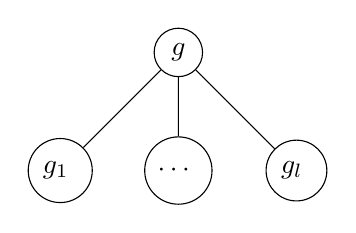
\begin{tikzpicture}[level distance=1.5cm,
  level 1/.style={sibling distance=1.5cm},
  every node/.style = {
  	shape=circle,
    draw,
    align=center,
    top color=white,
    bottom color=white
    }]
  \node {\( g \)}
    child {node { \( g_1 \) }}
    child {node { \( \cdots \) }}
    child {node { \( g_l \) }};
\end{tikzpicture}
\end{center}

For example, a circuit that encodes the function $f(a_1,a_2,a_3,a_4)=a_1a_2 +a_3a_4$ is 

\begin{center}
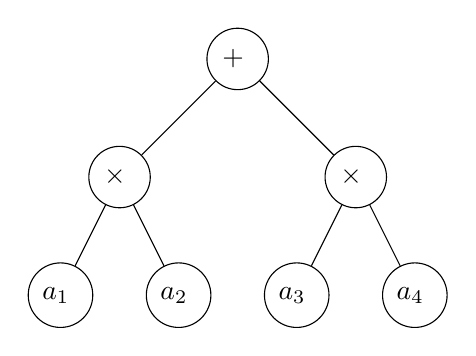
\begin{tikzpicture}[level distance=1.5cm,
  level 1/.style={sibling distance=3cm},
  level 2/.style={sibling distance=1.5cm},
  every node/.style = {
  	shape=circle,
    draw,
    align=center,
    top color=white,
    bottom color=white
    }
  ]
  \node { \( + \) }
    child { node { \( \times \) }
      child { node { \( a_1 \) } }
      child {node { \( a_2 \) } }
    }
    child { node { \( \times \) }
      child { node { \( a_3 \) } }
      child { node { \( a_4 \) } }
    };
\end{tikzpicture}
\end{center}

We can simulate the polynomial $x^2+xy$ by doing $f(A)$ where $A=[x \hspace{1ex} x \hspace{1ex} x \hspace{1ex} y]^*$. The main idea is to traverse the circuit top down in a depth first search way and store visited gates in a stack and its corresponding current values in another stack, and aggregate in the iterations according to the gate type.

For a stack $S$, the operations are standard:

\begin{itemize}
	\item $\push{S}{s}$: pushes $s$ into $S$.
	\item $\pop{S}$: pops the top element.
	\item $\getsize{S}$: the length of the stack.
	\item $\gettop{S}$: the top element in the stack.
\end{itemize}

For the pseudo-code, $\cG$ and $\cV$ denote stacks of gates and values, respectively. The property that holds during the simulation is that the value in $\cV[i]$ is the value that $\cG[i]$ currently outputs. The algorithm ends with $\cG=\left[ g_{\texttt{root}}\right]$ and $\cV=\left[ v_{\texttt{root}}\right]$ after traversing the circuit, and returns $v_{\texttt{root}}$

During the evaluation algorithm there will be two possible configurations of $\cG$ and $\cV$.

\begin{enumerate}
	\item $\getsize{\cG} = \getsize{\cV} + 1$: this means that $\gettop{\cG}$ is a gate that we visit for the first time and we need to initialize its value.
	
	\item $\getsize{\cG} = \getsize{\cV}$: here $\gettop{\cV}$ is the value of evaluating the circuit in gate $\gettop{\cG}$. Therefore, we need to aggregate the value $\gettop{\cV}$ to the parent gate of $g$.
\end{enumerate}

We assume the circuit has input gates, $+, \times$-gates and allow constant $1$-gate.

The idea is to traverse the circuit top down in a depth first search way. For example, in the circuit $f(a_1,a_2,a_3,a_4)=a_1a_2 +a_3a_4$ above, we would initialize the output gate value as $0$ because it is a $+$ gate, so $\cG=\lbrace +\rbrace$, $\cV=\lbrace 0\rbrace$. Then stack the left $\times$ gate to $\cG$, stack its initial value (i.e. $1$) to $\cV$. Now stack $a_1$ to $\cG$ and its value (i.e. $a_1$) to $\cV$. Since we are on an input gate we pop the gate and value pair off of $\cG$ and $\cV$ respectively, aggregate $a_1$ to $\gettop{\cV}$ and continue by stacking the $a_2$ gate to $\cG$. We pop $a_2$ off of $\cV$ (and its gate off of $\cG$) and aggregate its value to $\gettop{\cV}$. We pop and aggregate the value of the left $\times$ gate to $\gettop{\cV}$ (the root value). Then continue with the right $\times$ gate branch similarly.

For the pseudo-code, we supply ourselves with the following functions:

\begin{itemize}
	\item[--] $\isplus{g}$: true if and only if $g$ is a $+$-gate.
	\item[--] $\isprod{g}$: true if and only if $g$ is a $\times$-gate.
	\item[--] $\isone{g}$: true if and only if $g$ is a $1$-gate.
	\item[--] $\isinput{g}$: true if and only if $g$ is an input gate.
	\item[--] $\getfirst{g}$: outputs the first child of $g$.
	\item[--] $\getinput{g}$: outputs $A[i]$ when $g$ is the $i$-th input.
	\item[--] $\isnotlast{g_1}{g_2}$: true if and only if $g_2$ is not the last child gate of $g_1$.
	\item[--] $\nextgate{g_1}{g_2}$: outputs the next child gate of $g_1$ after $g_2$.
	\item[--] $\getroot$: outputs the root gate of the circuit.
\end{itemize}

The corresponding $\lbrace 0,1 \rbrace^n\rightarrow\lbrace 0,1 \rbrace^n$ functions are:

\begin{itemize}
	\item[--] $\isplus{g}$: $1$ if and only if $g$ is a $+$-gate.
	\item[--] $\isprod{g}$: $1$ if and only if $g$ is a $\times$-gate.
	\item[--] $\isone{g}$: $1$ if and only if $g$ is a $1$-gate.
	\item[--] $\isinput{g}$: $1$ if and only if $g$ is an input gate.
	\item[--] $\getfirst{g}$: outputs the $\texttt{id}$ of the first child of $g$.
	\item[--] $\getinput{g}$: outputs $e_i$ where the $i$-th input gate of $A$ is encoded by $g$.
	\item[--] $\isnotlast{g_1}{g_2}$: $1$ if and only if $g_2$ is not the last child gate of $g_1$.
	\item[--] $\nextgate{g_1}{g_2}$: outputs the $\texttt{id}$ of the next child gate of $g_1$ after $g_2$.
	\item[--] $\getroot$: outputs the $\texttt{id}$ of the root gate of the circuit.
\end{itemize}

The previous functions are all definable by an $L$-transducer and can be defined from the $L$-transducer of $f$. Then, by proposition \ref{prop:transducer}, for each of these functions there is a \langfor expression that simulates them.

Now, we give the pseudo-code of the top-down evaluation. We define the functions $Initialize$ (algorithm \ref{alg:init_code}), $Aggregate$ (algorithm \ref{alg:agg_code}) and $Evaluate$ (algorithm \ref{alg:eval_code}). The main algorithm is $Evaluate$.

\begin{algorithm}
\caption{Initialize (pseudo-code)}\label{alg:init_code}
\begin{algorithmic}[1]
\Function{Initialize}{$\cG, \cV, A$}\Comment{The stacks and input. Here, $\getsize{\cG} =  \getsize{\cV} + 1$}
	\If{$\isplus{\gettop{\cG}}$}
		\State $\push{\cV}{0}$
		\State $\push{\cG}{\getfirst{\gettop{\cG}}}$
	\ElsIf{$\isprod{\gettop{\cG}}$}
		\State $\push{\cV}{1}$
		\State $\push{\cG}{\getfirst{\gettop{\cG}}}$
	\ElsIf{$\isone{\gettop{\cG}}$}
		\State $\push{\cV}{1}$
	\ElsIf{$\isinput{\gettop{\cG}}$}
		\State $\push{\cV}{A\left[ \getinput{\gettop{\cG}} \right]}$
	\EndIf
	\State \textbf{return} $\cG, \cV$
\EndFunction
\end{algorithmic}
\end{algorithm}

\begin{algorithm}
\caption{Aggregate (pseudo-code)}\label{alg:agg_code}
\begin{algorithmic}[1]
\Function{Aggregate}{$\cG, \cV$}\Comment{Here, $\getsize{\cG} =  \getsize{\cV}$}
	\State $g = \pop{\cG}$
	\State $v = \pop{\cV}$
	\If{$\isplus{\gettop{\cG}}$}
		\State $\gettop{\cV} = \gettop{\cV} + v$
	\ElsIf{$\isprod{\gettop{\cG}}$}
		\State $\gettop{\cV} = \gettop{\cV} \cdot v$
	\EndIf
	\If{$\isnotlast{\gettop{\cG}}{g}$}
		\State $\push{\cG}{\nextgate{\gettop{\cG}}{g}}$
	\EndIf
	\State \textbf{return} $\cG, \cV$
\EndFunction
\end{algorithmic}
\end{algorithm}

\begin{algorithm}
\caption{Evaluate (pseudo-code)}\label{alg:eval_code}
\begin{algorithmic}[1]
\Function{Evaluate}{$A$}\Comment{Input $ n\times 1$ vector $A$. Here, $\cG$ and $\cV$ are empty}
	\State $\push{\cG}{\getroot}$
	\While{$\getsize{\cG}\neq 1$ or $\getsize{\cV}\neq 1$}
		\If{$\getsize{\cG}\neq \getsize{V}$}
			\State $(\cG,\cV) := \texttt{Initialize}(\cG,\cV,A)$
		\Else
			\State $(\cG,\cV):= \texttt{Aggregate}(\cG,\cV)$
		\EndIf
	\EndWhile
	\State \textbf{return} $\gettop{\cV}$
\EndFunction
\end{algorithmic}
\end{algorithm}

The $Evaluate$ algorithm gives us the output of the circuit. Note that after each iteration it either holds that $\getsize{\cG} =  \getsize{\cV} + 1$ or $\getsize{\cG} =  \getsize{\cV}$. Furthermore, when we start we have $\getsize{\cG}=1$ and $\getsize{\cV}=0$. The condition $\getsize{\cG}= 1$ and $\getsize{\cV}=1$ holds only when we have traversed all the circuit, and the value in $\gettop{\cV}$ is the value that the root of the circuit outputs after its computation.

Next, we show how to encode this algorithm in $\langfor$.

Let $n_0\in\mathbb{N}$ be big enough for $\star$ to hold and let $n\geq k$. Hence, the number of gates (values) is bounded by $n^k$ and we need $k\log (n)$ bits to encode the id of each gate.

To simulate the two stacks $\cG$ and $\cV$ we keep a matrix $X$ of dimensions $n \times n$.

\begin{itemize}
	\item Column $n$ will store a canonical vector that marks the top of stack $V$ (values).
	\item Column $n-1$ will store a canonical vector that marks the top of stack $G$ (gates).
	\item Column $n-2$ is the stack of values where $X[1, n-2]$ is the bottom of the stack.
	\item Columns $1$ to $n-3$ are the stack of gates.
\end{itemize}

If we have $j$ gates in the stack and currently $\getsize{\cG}=\getsize{\cV}$ then $X$ would look like:

\[
X = \begin{bmatrix}
    \texttt{id}_1 & v_1 & 0 & 0 \\
    \texttt{id}_2 & v_2 & 0 & 0 \\
    \vdots & \vdots & \vdots & \vdots \\
    \texttt{id}_j & v_j & 1 & 1 \\
    0 & 0 & 0 & 0 \\
    \vdots & \vdots & \vdots & \vdots \\
     0 & 0 & 0 & 0
\end{bmatrix}.
\]

Since $n\geq n_0$, $(\star)$ holds and thus we never use more than $n-3$ bits to encode an $\texttt{id}$. Also, $j\leq n$ given that we never keep more gates than the depth of the tree. As a consequence, we never keep more than $n$ values either.

\thomas{The following remark is necessary because of dimensions (check typing of START). I don't know if the reverse part is correct, but it makes sense to me since that way zeroes to the right actually mean nothing in the binary number (if it is reversed).}

An important detail is that the $\texttt{ids}$ of the gates are encoded as $\texttt{id}_r000$ for it to have dimension $n$, where $\texttt{id}_r$ is the corresponding binary number in reverse.

We make a series of definitions to make the notation more clear.

Let $e_i$ be the $i$-th canonical vector. $S$ and $P$ denote the successor and predecessor matrices respectively, such that

\[
  			S\cdot e_i=\begin{cases}
               e_{i+1} \text{ if } i\leq n \\
               \mathbf{0} \text{ otherwise }
            \end{cases}
\]

\[
  			P\cdot e_i=\begin{cases}
               e_{i-1} \text{ if } i\geq n \\
               \mathbf{0} \text{ otherwise }
            \end{cases}
\]

We write $e_{min}$ for the first canonical vector and $e_{max}$ for the last canonical vector. For any $i$ we write 
\begin{align*}
	e_{min+i} &= S^i\cdot e_{min} \\
	e_{max+i} &= P^i\cdot e_{max}
\end{align*}

We use the extra $\lbrace 0,1 \rbrace^n\rightarrow\lbrace 0,1 \rbrace^n$ functions that have a $\langfor$ translation:

\[
  			min(e)=\begin{cases}
               1 \text{ if } e=e_{min} \\
               0 \text{ otherwise }
             \end{cases}
\]

\[
  			max(e)=\begin{cases}
               1 \text{ if } e=e_{max} \\
               0 \text{ otherwise }
             \end{cases}
\]

\[
  			less(e_i,e_j)=\begin{cases}
               1 \text{ if } i\leq j \\
               0 \text{ otherwise }
             \end{cases}
\]

When used in $\langfor$ these functions output $[0]$ and $[1]$.

Now 
\begin{align*}
	e_{V}&:=e_{max-2} \\
	e_{G_{top}}&:=e_{max-1} \\
	e_{V_{top}}&:=e_{max}
\end{align*}

For a canonical vector, let $$\Iden{e_i}:=\ssum v. less(v,e_i)\cdot (v\cdot v^*).$$ This matrix has ones in the diagonal up to position $i$ marked by $e_{i}$. We define the following sub-matrices of $X$:
\begin{align*}
	V_{top} &:= X\cdot e_{V_{top}} \\
	V &:= \Iden{V_{top}} \cdot X \cdot e_v \\
 	G_{top} &:=X\cdot e_{G_{top}} \\
 	G &:= \Iden{G_{top}}\cdot X \cdot \Iden{e_{max-3}}
\end{align*}

For example, if we are in a step where $\getsize{\cG}=\getsize{\cV} + 1$ then

\[
X = \begin{bmatrix}
    \texttt{id}_1 & v_1 & 0 & 0 \\
    \texttt{id}_2 & v_2 & 0 & 0 \\
    \vdots & \vdots & \vdots & \vdots \\
    \texttt{id}_{j-1} & v_{j-1} & 0 & 1 \\
    \texttt{id}_j & 0 & 1 & 0 \\
    0 & 0 & 0 & 0 \\
    \vdots & \vdots & \vdots & \vdots \\
     0 & 0 & 0 & 0
\end{bmatrix}, 
G = \begin{bmatrix}
    \texttt{id}_1  \\
    \texttt{id}_2 \\
    \vdots   \\
    \texttt{id}_{j-1} \\
    \texttt{id}_j \\
    0 \\
    \vdots \\
     0 
\end{bmatrix}, 
V = \begin{bmatrix}
    v_1  \\
    v_2 \\
    \vdots   \\
    v_{j-1} \\
    0 \\
    0 \\
    \vdots \\
     0 
\end{bmatrix}, 
G_{top} = \begin{bmatrix}
    0  \\
    0 \\
    \vdots   \\
    0 \\
    1 \\
    0 \\
    \vdots \\
     0 
\end{bmatrix}, 
V_{top} = \begin{bmatrix}
    0  \\
    0 \\
    \vdots   \\
    1 \\
    0 \\
    0 \\
    \vdots \\
     0 
\end{bmatrix}
\]

Here, $V$ is a vector encoding the stack of values in $X$ and $G$ is a matrix encoding the stack of gates in $X$. Note that what is \textit{over} the top of the stacks is always set to zero due to $\Iden{G_{top}}$ and $\Iden{V_{top}}$.

To set the initial state (algorithm \ref{alg:eval_code} line 2) we define the $\langfor$ expression: $$\text{START}:= e_{min}\cdot \getroot^* + e_{min}\cdot e_{G_{top}}^*.$$
For the initialize step, we define the $\langfor$ expressions: INIT${\_}$PLUS (algorithm \ref{alg:init_code}, lines 2, 3, 4), INIT${\_}$PROD (algorithm \ref{alg:init_code}, lines 5, 6, 7), CONST (algorithm \ref{alg:init_code}, lines 8, 9) and INPUT (algorithm \ref{alg:init_code}, lines 10, 11):

\begin{align*}
	\text{INIT{\_}PLUS} &:= \isplus{G^*\cdot G_{top}}\odot \left[ G + S\cdot G_{top} \cdot \getfirst{G^*\cdot G_{top}}^*  + S\cdot G_{top}\cdot e_{G_{top}}^* +V\cdot e_{V} + S\cdot V_{top}\cdot e_{V_{top}}^* \right] \\
	\text{INIT{\_}PROD} &:= \isprod{G^*\cdot G_{top}}\odot \left[ G + S\cdot G_{top} \cdot \getfirst{G^*\cdot G_{top}}^* + S\cdot G_{top}\cdot e_{G_{top}}^* +(V + S\cdot v_{top})\cdot e_{V} + S\cdot V_{top}\cdot e_{V_{top}}^* \right] \\
	\text{CONST} &:= \isone{G^*\cdot G_{top}}\odot \left[ G + (V + S\cdot v_{top})\cdot e_{V} + S\cdot V_{top}\cdot e_{V_{top}}^* \right] \\
	\text{INPUT} &:= \isinput{G^*\cdot G_{top}}\odot \left[ G + \left(V + \left( A^* \cdot \getinput{G^*\cdot G_{top}} \cdot S\cdot V_{top} \right)\right)\cdot e_{V} + S\cdot V_{top}\cdot e_{V_{top}}^* \right]
\end{align*} 

Here, $G^*\cdot G_{top}$ is to get the current id in the top of the stack. In INIT${\_}$PLUS we get the current stack $G$, we add $S\cdot G_{top} \cdot \getfirst{G^*\cdot G_{top}}^*$ which is an $n\times n$ matrix with the first child of $G^*\cdot G_{top}$ in the next row. Then $S\cdot G_{top}\cdot e_{G_{top}}^*$ adds $S\cdot G_{top}$ to the $n-1$ column to mark the gate we added as the top. Next, we do the same with the values by adding $V\cdot e_{V} + S\cdot V_{top}\cdot e_{V_{top}}^*$.

The $\langfor$ expression equivalent to algorithm \ref{alg:init_code} is $$\text{INIT}:=\text{INIT{\_}PLUS}+\text{INIT{\_}PROD}+\text{CONST}+\text{INPUT}.$$

The idea is to return the matrix for the next iteration. Recall that here $\getsize{\cG}=\getsize{\cV} + 1$. So, when the operation is INPUT or CONST, if we start with

\[
\begin{bmatrix}
    \texttt{id}_1 & v_1 & 0 & 0 \\
    \texttt{id}_2 & v_2 & 0 & 0 \\
    \vdots & \vdots & \vdots & \vdots \\
    \texttt{id}_{j-1} & v_{j-1} & 0 & 1 \\
    \texttt{id}_j & 0 & 1 & 0 \\
    0 & 0 & 0 & 0 \\
    \vdots & \vdots & \vdots & \vdots \\
     0 & 0 & 0 & 0
\end{bmatrix}, \text{ then we return }
\begin{bmatrix}
    \texttt{id}_1 & v_1 & 0 & 0 \\
    \texttt{id}_2 & v_2 & 0 & 0 \\
    \vdots & \vdots & \vdots & \vdots \\
    \texttt{id}_{j-1} & v_{j-1} & 0 & 0 \\
    \texttt{id}_j & v_j & 1 & 1 \\
    0 & 0 & 0 & 0 \\
    \vdots & \vdots & \vdots & \vdots \\
     0 & 0 & 0 & 0
\end{bmatrix}.
\]

When the operation is INIT{\_}PLUS or INIT{\_}PROD, if we start with 

\[
\begin{bmatrix}
    \texttt{id}_1 & v_1 & 0 & 0 \\
    \texttt{id}_2 & v_2 & 0 & 0 \\
    \vdots & \vdots & \vdots & \vdots \\
    \texttt{id}_{j-1} & v_{j-1} & 0 & 1 \\
    \texttt{id}_j & 0 & 1 & 0 \\
    0 & 0 & 0 & 0 \\
    0 & 0 & 0 & 0 \\
    \vdots & \vdots & \vdots & \vdots \\
     0 & 0 & 0 & 0
\end{bmatrix}, \text{ then we return }
\begin{bmatrix}
    \texttt{id}_1 & v_1 & 0 & 0 \\
    \texttt{id}_2 & v_2 & 0 & 0 \\
    \vdots & \vdots & \vdots & \vdots \\
    \texttt{id}_{j-1} & v_{j-1} & 0 & 0 \\
    \texttt{id}_j & v_j & 0 & 1 \\
    \texttt{id}_{j+1} & 0 & 1 & 0 \\
    0 & 0 & 0 & 0 \\
    \vdots & \vdots & \vdots & \vdots \\
     0 & 0 & 0 & 0
\end{bmatrix}.
\]


For the aggregate expression (algorithm \ref{alg:agg_code}) we do the following. Let $$\pondIden{e_i}{c}=\ssum v. (v^*\cdot e_i)\cdot c\cdot v\cdot v^* + (1-v^*\cdot e_i)\cdot v \cdot v^*,$$ namely, it is the identity with $c$ in position $(i,i)$.

We define the expressions: AGG${\_}$PLUS (algorithm \ref{alg:agg_code}, lines 4, 5), AGG${\_}$PROD (algorithm \ref{alg:agg_code}, lines 6, 7),  IS${\_}$NOT${\_}$LAST (algorithm \ref{alg:agg_code}, lines 8, 9), IS${\_}$LAST and POP:

\begin{align*}
	\text{POP} &:= \Iden{P\cdot G_{top}}\cdot G + P\cdot V_{top}\cdot e_{V_{top}}^*  \\
	\text{AGG{\_}PLUS} &:= \isplus{G^* \cdot \left( P \cdot G_{top}\right)} \odot \left[ \left( \Iden{P\cdot V_{top}} \cdot V + \left( V^* \cdot V_{top} \right)\left( P\cdot V_{top} \right)\right) \cdot e_{V}^* \right] \\
	\text{AGG{\_}PROD} &:= \isprod{G^* \cdot \left( P \cdot G_{top}\right)} \odot \left[ \left( \pondIden{P\cdot V_{top}}{V^* \cdot V_{top}} \cdot \Iden{P\cdot V_{top}} \cdot V \right) \cdot e_{V}^* \right] \\
	\text{IS{\_}NOT{\_}LAST} &:= \isnotlast{G^* \cdot \left( P \cdot G_{top}\right)}{G^* \cdot G_{top}} \odot \left[  G_{top} \cdot \nextgate{G^* \cdot \left( P\cdot G_{top} \right) }{G^* \cdot G_{top}} + G_{top}\cdot e_{G_{top}}^* \right] \\
	\text{IS{\_}LAST} &:= \left( 1 - \isnotlast{G^* \cdot \left( P \cdot G_{top}\right)}{G^* \cdot G_{top}} \right)\odot \left[ \left( P\cdot G_{top} \right) \cdot e_{G_{top}}^* \right]
\end{align*}

The $\langfor$ expression equivalent to algorithm \ref{alg:agg_code} is $$\text{AGG}:=\text{POP} + \text{AGG{\_}PLUS}+\text{AGG{\_}PROD}+\text{IS{\_}NOT{\_}LAST}+\text{IS{\_}LAST}.$$

The $Evaluate$ method (algorithm \ref{alg:eval_code}) is defined as follows:

\begin{align*}
	\text{EVAL}&[A]= \\
	&e_{min}^* \cdot \ffor{X}{v_1, \ldots, v_k}: \big\lbrace \\
	&\left( \sprod_{i=1}^k min(v_i)\right) \odot START + \\
	&\left( 1- \sprod_{i=1}^k min(v_i)\right) \odot \left( \left(1 - min(G_{top})\cdot min(V_{top}) \right) \odot \left[ \left( 1 - G_{top}^*\cdot V_{top} \right) \odot \text{INIT} + \left(  G_{top}^*\cdot V_{top} \right) \odot \text{AGG} \right] + min(G_{top})\odot min(V_{top})\odot X\right) \\ 
	&\big\rbrace \cdot e_{V}
\end{align*}

Note that the $ \texttt{for}$-expression does the evaluation. The final output is in $X[1,max-2]$, we extract this value by multiplying the final result as $e_{min}^*\cdot [\texttt{for}(\ldots )]\cdot e_{V}$.

Finally, we need to take care of all $n<n_0$, where $(\star)$ does not necessarily hold. For any $i$, let: $$\text{Eval}[i,A]:= \text{ the } 1\times 1 \text{ matrix with the value of the polynomial } f(A) \text{ when } n=i.$$

Then we define: $$f(A)=\ssum_{i=0}^{n_0-1}(e_{min+i}\cdot e_{max}^*)\odot \text{EVAL}[i,A] + \left( (S^{n_0}\cdot e_{min})^*\cdot \ones (e_{min}) \right)\odot \text{EVAL}[A].$$ Above, $(e_{min+i}\cdot e_{max}^*)$ checks if the dimension is equal to $i$, and $(S^{n_0}\cdot e_{min})^*\cdot \ones (e_{min})$ checks if the dimension is greater or equal than $n_0$.














\subsection{From MATLANG to uniform ACs}
% We connect MATLANG with arithmetic circuits as follows.

% We first show that for every MATLANG expression $e$ we can associate a uniform arithmetic circuit family $\{\Phi_n^e\mid n=1,2,\ldots\}$ such that when $I$ is matrix instance of dimension $n$ (or $n\times n$), we can obtain $e(I)$ by evaluating $\Phi_n$ on $I$. \floris{The connection between the dimensions of instances etc and the ``$n$'' in the arithmetic circuits needs to be made precise. E.g., if we have $n^2$ matrices, we need more than $n$ variables...}

We consider circuits over matrices (multiple output gates). We will write 
$\Phi(A_1,\ldots ,A_k)$, where $\Phi$ is an arithmetic circuit with multiple output gates, and each 
$A_i$ is a matrix of dimensions $\alpha_i\times \beta_i$, with $\alpha_i,\beta_i \in \{n,1\}$ to denote 
the input matrices for a circuit $\Phi$. We will also write $\ttype(\Phi)=(\alpha,\beta)$, with 
$\alpha,\beta\in \{n,1\}$, to denote the size of the output matrix for $\Phi$. 
When $\{\Phi_n\mid n=1,2,\ldots\}$ is a uniform family of 
arithmetic circuits over matrices, we will assume that the Turing machine for generating $\Phi_n$ also 
gives us the information about how to access a position of each input matrix, and how to access the 
positions of the output matrix, as is usually done when handling matrices with arithmetic 
circuits \cite{Raz02}. The notion of degree is extended to be the sum of the degrees of all 
the output gates. The former will be denoted as $\Phi_{n}[i,j]$ when $\ttype(\Phi)=(n,n)$, 
$\Phi_{n}[i,1]$ when $\ttype(\Phi)=(n,1)$, $\Phi_{n}[1,j]$ when $\ttype(\Phi)=(1,n)$ and 
$\Phi_{n}$ when $\ttype(\Phi)=(1,1)$. Also, when we write $a \oplus b$ we mean 

\begin{center}
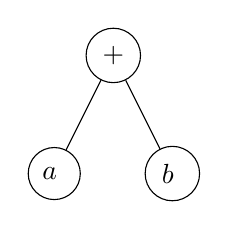
\begin{tikzpicture}[level distance=1.5cm,
  level 1/.style={sibling distance=1.5cm},
  every node/.style = {
  	shape=circle,
    draw,
    align=center,
    top color=white,
    bottom color=white
    }]
  \node {\( + \)}
    child {node { \( a \) }}
    child {node { \( b \) }};
\end{tikzpicture}
\end{center}
When we write $\bigoplus_{l=1}^n a_l$ we mean 

\begin{center}
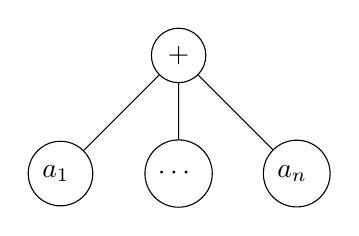
\begin{tikzpicture}[level distance=1.5cm,
  level 1/.style={sibling distance=1.5cm},
  every node/.style = {
  	shape=circle,
    draw,
    align=center,
    top color=white,
    bottom color=white
    }]
  \node {\( + \)}
    child {node { \( a_1 \) }}
    child {node { \( \cdots \) }}
    child {node { \( a_n \) }};
\end{tikzpicture}
\end{center}
Same with $\otimes$. Now we prove the statement.

\newtheorem*{LANGINCIRC}{Theorem~\ref{th-ml-to-circuits}}

\begin{LANGINCIRC}
  Let $e$ be a \langfor expression over a schema $\Sch$, and let $V_1,\ldots ,V_k$ be the variables of $e$ such that $\ttype(V_i)\in \{(\alpha,\alpha), (\alpha,1), (1,\alpha), (1,1)\}$. Then there exists a uniform arithmetic circuit family over matrices $\Phi_n(A_1,\ldots ,A_k)$ such that:
  \begin{itemize}
  \item For any instance $\I = (\dom,\conc)$ such that $\dom(\alpha) = n$ and $\conc(V_i) = A_i$ it holds that:
  \item $\sem{e}{\I} = \Phi_n(A_1,\ldots ,A_k)$.
  \end{itemize}
\end{LANGINCIRC}


\begin{proof}

Let $e$ be a \langfor expression. 

If $e=V$ then $\Phi_n^e:=\Phi(A)$, and we have that
\begin{itemize}
	\item If $\ttype(V)=(1,1)$ then $\ttype(\Phi^e_n)=(1,1)$ and $\Phi^e_n$ has the one input/output gate.
	\item If $\ttype(V)=(1,\alpha)$ then $\ttype(\Phi^e_n)=(1,n)$ and $\Phi^e_n$ has $n$ input/output gates.
  \item If $\ttype(V)=(\alpha,1)$ then $\ttype(\Phi^e_n)=(n,1)$ and $\Phi^e_n$ has $n$ input/output gates.
	\item If $\ttype(V)=(\alpha,\alpha)$ then $\ttype(\Phi^e_n)=(n,n)$ and $\Phi^e_n$ has $n^2$ input/output gates. $\Phi^e_n$ has $n^2$ input/output gates.
\end{itemize}

If $e=e'^T$ then $\Phi^e_n=\Phi^{e'}_n$. 
\begin{itemize}
	\item If $\ttype(\Phi^{e'}_n)=(1, 1)$ then$\Phi^e_n=\Phi^{e'}_n$ and $\type(\Phi^e_n)=(1,1)$.
	\item If $\ttype(\Phi^{e'}_n)=(1, n)$ then $\type(\Phi^e_n)=(n,1)$ and $\Phi^e_n[i,1]:=\Phi^{e'}_n[1,i]$. 
  \item If $\ttype(\Phi^{e'}_n)=(n, 1)$ then $\type(\Phi^e_n)=(1,n)$ and $\Phi^e_n[1,j]:=\Phi^{e'}_n[j,1]$. 
  \item If $\ttype(\Phi^{e'}_n)=(n, n)$ then $\type(\Phi^e_n)=(n,n)$ and $\Phi^e_n[i,j]:=\Phi^{e'}_n[j,i]$. 
\end{itemize}

If $e=e_{\ones}(e')$ where $\ttype(\Phi^{e'}_n)=(\alpha,\beta)$ then $\ttype(\Phi^{e}_n)=(\alpha,1)$ and $\Phi^e_n[i,1]:=1$.

If $e=e_1 + e_2$ we have

\begin{itemize}
	\item When $\ttype(\Phi^{e_1}_n)=\ttype(\Phi^{e_2}_n)=(1, 1)$ is then $\ttype(\Phi^{e}_n)=(1, 1)$ and $\Phi^e_n:=\Phi^{e_1}_n \oplus \Phi^{e_2}_n$.
  \item When $\ttype(\Phi^{e_1}_n)=\ttype(\Phi^{e_2}_n)=(1, n)$ is then $\ttype(\Phi^{e}_n)=(1, n)$ and $\Phi^e_n[1,j]:=\Phi^{e_1}_n[1,j] \oplus \Phi^{e_2}_n[1,j]$.
  \item When $\ttype(\Phi^{e_1}_n)=\ttype(\Phi^{e_2}_n)=(n, 1)$ is then $\ttype(\Phi^{e}_n)=(n, 1)$ and $\Phi^e_n[i,1]:=\Phi^{e_1}_n[i,1] \oplus \Phi^{e_2}_n[i,1]$.
  \item When $\ttype(\Phi^{e_1}_n)=\ttype(\Phi^{e_2}_n)=(n, n)$ is then $\ttype(\Phi^{e}_n)=(n, n)$ and $\Phi^e_n[i,j]:=\Phi^{e_1}_n[i,j] \oplus \Phi^{e_2}_n[i,j]$.
\end{itemize}

If $e=f(e_1, \ldots, e_k)$ we have two cases

\begin{itemize}
  \item When $f$ is retricted to $f_{\odot}$ then
  \begin{itemize}
    \item If $\ttype(\Phi^{e_1}_n)=\ldots =\ttype(\Phi^{e_k}_n)=(1, 1)$ then $\Phi^e_n:=\bigotimes_{l=1}^k \Phi^{e_l}_n$.
    \item If $\ttype(\Phi^{e_1}_n)=\ldots =\ttype(\Phi^{e_k}_n)=(1, n)$ then $\Phi^e_n[1,j]:=\bigotimes_{l=1}^k \Phi^{e_l}_n[1,j]$.
    \item If $\ttype(\Phi^{e_1}_n)=\ldots =\ttype(\Phi^{e_k}_n)=(n, 1)$ then $\Phi^e_n[i,1]:=\bigotimes_{l=1}^k \Phi^{e_l}_n[i,1]$.
    \item If $\ttype(\Phi^{e_1}_n)=\ldots =\ttype(\Phi^{e_k}_n)=(n, n)$ then $\Phi^e_n[i,j]:=\bigotimes_{l=1}^k \Phi^{e_l}_n[i,j]$.
  \end{itemize}
	\item When $f$ is any function, we prove the case when $\ttype(\Phi^{e_1}_n)=\ldots =\ttype(\Phi^{e_k}_n)=(1, 1)$
  (only case necessary). Here $\Phi^e_n$ is 
	
\begin{center}
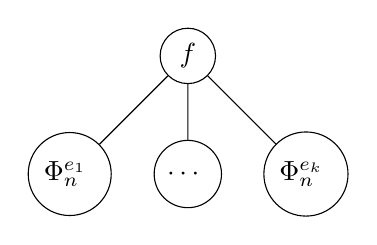
\begin{tikzpicture}[level distance=1.5cm,
  level 1/.style={sibling distance=1.5cm},
  every node/.style = {
  	shape=circle,
    draw,
    align=center,
    top color=white,
    bottom color=white
    }]
  \node {\( f \)}
    child {node { \( \Phi^{e_1}_n \) }}
    child {node { \( \cdots \) }}
    child {node { \( \Phi^{e_k}_n \) }};
\end{tikzpicture}
\end{center}

\end{itemize}

If $e=e_1\cdot e_2$ we have

\begin{itemize}
	\item When $\ttype(\Phi^{e_1}_n)=(1,1)$ and $\ttype(\Phi^{e_2}_n)=(1, 1)$ then $\ttype(\Phi^{e}_n)=(1, 1)$ and $\Phi^{e}_n:=\Phi^{e_1}_n \otimes \Phi^{e_2}_n$.
  \item When $\ttype(\Phi^{e_1}_n)=(1,1)$ and $\ttype(\Phi^{e_2}_n)=(1, n)$ then $\ttype(\Phi^{e}_n)=(1, n)$ and $\Phi^{e}_n[1,j]:=\Phi^{e_1}_n \otimes \Phi^{e_2}_n[1,j]$.
  \item When $\ttype(\Phi^{e_1}_n)=(n,1)$ and $\ttype(\Phi^{e_2}_n)=(1, 1)$ then $\ttype(\Phi^{e}_n)=(n, 1)$ and $\Phi^{e}_n[i,1]:=\Phi^{e_1}_n[i,1] \otimes \Phi^{e_2}_n$.
  \item When $\ttype(\Phi^{e_1}_n)=(n,1)$ and $\ttype(\Phi^{e_2}_n)=(1, n)$ then $\ttype(\Phi^{e}_n)=(n, n)$ and $\Phi^{e}_n[i,j]:=\Phi^{e_1}_n[i,1] \otimes \Phi^{e_2}_n[1,j]$.
  \item When $\ttype(\Phi^{e_1}_n)=(1,n)$ and $\ttype(\Phi^{e_2}_n)=(n, 1)$ then $\ttype(\Phi^{e}_n)=(1, 1)$ and $$\Phi^{e}_n:=\bigoplus_{k=1}^n \left( \Phi^{e_1}_n[1,k] \otimes \Phi^{e_2}_n[k,1] \right).$$
  \item When $\ttype(\Phi^{e_1}_n)=(1,n)$ and $\ttype(\Phi^{e_2}_n)=(n, n)$ then $\ttype(\Phi^{e}_n)=(1, n)$ and $$\Phi^{e}_n[1,j]:=\bigoplus_{k=1}^n \left( \Phi^{e_1}_n[1,k] \otimes \Phi^{e_2}_n[k,j] \right).$$
  \item When $\ttype(\Phi^{e_1}_n)=(n,n)$ and $\ttype(\Phi^{e_2}_n)=(n, 1)$ then $\ttype(\Phi^{e}_n)=(n, 1)$ and $$\Phi^{e}_n[i,1]:=\bigoplus_{k=1}^n \left( \Phi^{e_1}_n[i,k] \otimes \Phi^{e_2}_n[k,1] \right).$$
  \item When $\ttype(\Phi^{e_1}_n)=(n,n)$ and $\ttype(\Phi^{e_2}_n)=(n, n)$ then $\ttype(\Phi^{e}_n)=(n, n)$ and $$\Phi^{e}_n[i,j]:=\bigoplus_{k=1}^n \left( \Phi^{e_1}_n[i,k] \otimes \Phi^{e_2}_n[k,j] \right).$$
\end{itemize}

If $e=\ffor{X}{v}e'(X, v)$, then define $\Phi^{\mathbf{0}}$ 
as the zero matrix circuit $\ttype(\Phi^{\mathbf{0}})=(1,1)$ if $\ttype(\Phi^{e'}_n)=(1,1)$ and 
$\ttype(\Phi^{\mathbf{0}})=(n,n)$ if $\ttype(\Phi^{e'}_n)=(n,n)$. Also, $\Phi^{\mathbf{0}}=0$ and
$\Phi^{\mathbf{0}}[i,j]=0$ $\forall i,j$ for each case respectively. Now for $i=1,\ldots, n$, define
$\Phi^{v_i}$ as the circuit such that $\ttype(\Phi^{v_i})=(n,1)$ and $\Phi^{v_i}[i,1]:=1$ and zero otherwise.
Finally, define

$$\Phi^{e}_n=\Phi^{e'}_n\left( \Phi^{e'}_n \left( \cdots \left( \Phi^{e'}_n\left( \Phi^{\mathbf{0}}, \Phi^{v_1}\right), \Phi^{v_2}\right)\cdots, \Phi^{v_{n-1}} \right), \Phi^{v_n} \right).$$

Note that every circuit adds a constant number of layers except when $e=\ffor{X}{v}e'(X, v)$. 
This means that the depth still is polynomial. When $e=\ffor{X}{v}e'(X, v)$
we have that the depth of the circuit is $n\cdot p(n)$, where the depth of $e'(X, v)$ is $p(n)$, 
so it also remains polynomial.

Here, we do not need to translate scalar multiplication
because it can be simulated using the $\mathsf{ones}$ operator and $f_{\kprod}$ (see section \ref{app:simp}).

\end{proof}

% As a consequence, blah blah....

% In general, uniform arithmetic circuit family $\{\Phi_n^e\mid n=1,2,\ldots\}$ is not necessarily of polynomial degree. Indeed, consider it suffices to consider the MATLANG expression which computes
% $f_n(x)=x^{2^n}$. 
% As uniform arithmetic circuit families of polynomial degree have nice properties, e.g., they can be assumed to be of logarithmic depth, we next want to zoom in such families. In what follows we therefore limit ourselves to MATLANG expressions $e$ such that $\{\Phi_n^e\mid n=1,2,\ldots\}$ is a family of polynomial degree arithmetic circuits.

% \begin{itemize}
% 	\item Checking whether a MATLANG expression $e$ corresponds to a family of of polynomial degree arithmetic circuits is undecidable. 
% \end{itemize}

% Let $e$ be a ``nice'' MATLANG expression, i.e.,  $\{\Phi_n^e\mid n=1,2,\ldots\}$ is a family of polynomial degree arithmetic circuits which can be assumed to be logarithmic depth. 
% \begin{itemize}
% 	\item There exists a MATLANG expression that can
% \end{itemize}

% Let $e$ be a \langfor expression. If $e=V$ we have
% \begin{itemize}
% 	\item When $V$ is $1\times 1$ then $\Phi^e_1$ has the one input/output gate (\textit{not necessary, covered in second item}).
% 	\item When $V$ is $n\times 1$ or $1\times n$ then $\Phi^e_n$ has $n$ input/output gates.
% 	\item When $V$ is $n\times n$ then $\Phi^e_n$ has $n^2$ input/output gates. Here, $V_{ij}=\Phi_n(V)\left[ j+n(i-1)\right]$ and $i,j=1,\ldots, n$ (entries listed row by row).
% \end{itemize}

% If $e=e'^T$ then $\Phi^e_n=\Phi^{e'}_n$. 

% If $e=e_1 + e_2$ we have

% \begin{itemize}
% 	\item When $e$ is $1\times 1$ then $\Phi^e_1$ is $\Phi^{e_1}_1 \oplus \Phi^{e_2}_1$.
% 	\item When $e$ is $n\times 1$ or $1\times n$ then $\Phi^e_n$ has $n$ output gates, where gate $k$ is $\Phi^{e_1}_n[k] \oplus \Phi^{e_2}_n[k]$.
% 	\item When $V$ is $n\times n$ then $\Phi^e_1$ has $n^2$ output gates, where gate $k$ is $\Phi^{e_1}_n[k] \oplus \Phi^{e_2}_n[k]$.
% \end{itemize}

% If $e=f(e_1, \ldots, e_k)$ we have

% \begin{itemize}
% 	\item When $e$ is $1\times 1$ (only case necessary) then $\Phi^e_1$ is 
	
% \begin{center}
% \begin{tikzpicture}[level distance=1.5cm,
%   level 1/.style={sibling distance=1.5cm},
%   every node/.style = {
%   	shape=circle,
%     draw,
%     align=center,
%     top color=white,
%     bottom color=white
%     }]
%   \node {\( f \)}
%     child {node { \( \Phi^{e_1}_1 \) }}
%     child {node { \( \cdots \) }}
%     child {node { \( \Phi^{e_k}_1 \) }};
% \end{tikzpicture}
% \end{center}

% \end{itemize}

% If $e=e_1\cdot e_2$ we have

% \begin{itemize}
% 	\item When $e_1,e_2$ are $1\times 1$ then $\Phi^e_1$ is $\Phi^{e_1}_1 \otimes \Phi^{e_2}_1$.
% 	\item When $e_1$ is $1\times 1$ and $e_2$ is $1\times n$ then $\Phi^e_n$ has $n$ output gates, where output gate $i$ is $\Phi^{e_1}_1 \otimes \Phi^{e_2}_n[i]$.
% 	\item When $e_1$ is $n\times 1$ and $e_2$ is $1\times 1$ then $\Phi^e_n$ has $n$ output gates, where output gate $i$ is $\Phi^{e_1}_n[i] \otimes \Phi^{e_2}_1$.
% 	\item When $e_1$ is $n\times 1$ and $e_2$ is $1\times n$ then $\Phi^e_n$ has $n^2$ output gates, where output gate $k=j + n(i-1)$ is $\Phi^{e_1}_n[i] \otimes \Phi^{e_2}_n[j]$. Note that $k=1,\ldots, n^2$ and $i,j=1,\ldots, n$.
% 	\item When $e_1$ is $1\times n$ and $e_2$ is $n\times 1$ then $\Phi^e_n$ has one output gate $$\bigoplus_{l=1}^n \left( \Phi^{e_1}_n[l] \otimes \Phi^{e_2}_n[l] \right).$$
% 	\item When $e_1$ is $1\times n$ and $e_2$ is $n\times n$ then $\Phi^e_n$ has $n$ output gates, where gate $j$ is $$\bigoplus_{i=1}^n \left( \Phi^{e_1}_n[j] \otimes \Phi^{e_2}_n[j + n(i-1)] \right).$$
% 	\item When $e_1$ is $n\times n$ and $e_2$ is $n\times 1$ then $\Phi^e_n$ has $n$ output gates, where gate $i$ is $$\bigoplus_{j=1}^n \left( \Phi^{e_1}_n[j+n(i-1)] \otimes \Phi^{e_2}_n[j] \right).$$
% 	\item When $e_1$ is $n\times n$ and $e_2$ is $n\times n$ then $\Phi^e_n$ has $n^2$ output gates, where gate $k=j+n(i-1)$ is $$\bigoplus_{l=1}^n \left( \Phi^{e_1}_n[i] \otimes \Phi^{e_2}_n[j+n(l-1)] \right).$$ Note that $k=1,\ldots, n^2$ and $i,j=1,\ldots, n$.
% \end{itemize}

% If $e=\ffor{X}{v}e'(\cI, X, v)$ then $$\Phi^{e}_n=\Phi^{e'}_n\left( \cI, \Phi^{e'}_n \left( \cI, \cdots \Phi^{e'}_n\left( \cI, \Phi^{e'}_n\left( \cI, 0, v_1\right), v_2\right)\cdots, v_{n-1} \right), v_n \right).$$

% Note that every circuit adds a constant number of layers except when $e=\ffor{X}{v}e'(\cI, X, v)$. This means that the depth still is polynomial. When $e=\ffor{X}{v}e'(\cI, X, v)$ we have that the depth of the circuit is $n\cdot p(n)$, where the depth of $e'(\cI, X, v)$ is $p(n)$, so it also remains polynomial.

\subsection{Undecidability}
%!TEX root = /Users/fgeerts/Documents/MLforloops/pods/main.tex

\floris{Not finished...}
In this section we consider the problem of deciding the class
$$
\{ e\in \mathsf{MATLANG}\mid\text{$\{\Phi_n^e\mid n=1,2,\ldots\}$ is of polynomial degree}\},
$$
where $\{\Phi_n^e\mid n=1,2,\ldots\}$ denotes the uniform family of arithmetic circuits associated with $e$.
We show that this problem is undecidable. To see this, we use that the problem of deciding the class
$$
\{ \langle M\rangle\mid \text{$M$ is a deterministic TM which halts on the empty input}\}
$$
is undecidable. Consider a TM $M$ described by $(Q,\Gamma=\{0,1\},q_0,q_m,\Delta)$
with $Q=\{q_1,\ldots,q_m\}$ its states, $q_1$ being the initial state and $q_m$ being
the halting state, $\Gamma$ is the tape alphabet, and $\Delta$ is a transition function
from $Q\times \Gamma\to Q\times\Gamma\times \{\leftarrow,\sqcup,\rightarrow\}$. The 
simulation by a MATLANG expression of a linear space TM can be easily modified to
any TM $M$ provided that we limit the execution of $M$ to exactly $n$ steps. Similarly
as in the linear space TM simulation, we have relation $Q_1,\ldots,Q_m$ encoding the
states, a single relation $T$ encoding the tape and relation $H_T$ encoding the position
of the tape. We note that we do not have any input so when initialising the matrices
for these relations, we can use a tape of size $n$. By contrast to the linear space 
simulation, we also use a single vector $v$ (instead of $k$ such vectors) 
to simulate $n$ steps of $M$. We modify the expression such that it return $0$ if $M$
halts in at most $n$ steps, and $1$ if $M$ did not halt yet after $n$ steps.

As a consequence, when $M$ halts, there is a $N$ such that our MATLANG expression
$e_M$ will return $1$ when the relations have dimension $n\geq N$. Otherwise, when
$M$ does not halt, we have that $e_M$ returns $0$ for all dimensions. It now suffices
to consider the matlang expression
$$
d_M:=e_M\cdot e_{2^x}
$$
where $e_{2^x}$ computes the functions $2^{2^n}$. If we let 
$\Phi_n$ denote the circuit corresponding to $d_M$ for dimension $n$,
then this will be a polynomial degree family of circuits if 
 $e_{2^x}$ is called only



%
% 3/ Based on e_M(n) we now consider the ML expression
%
%  d_M(n):=e_M(n) Pow(n)
%
% with Pow(n)=2^n (or any other ML expression which cannot
% be computed by a poly degree circuit). Then, d_M(n) will be of
% poly degree if M does not halt in n steps. And since we
% want to know whether it is poly degree for all n (uniform circuits)
% M should not halt. Hence, the poly degree problem cannot be decidable.



\section{Proofs of Section~\ref{sec:restrict}}

\subsection{From \langsum to ARA}
\newtheorem*{SUMTOARA}{Proposition~\ref{prop:sum_to_ara}}

We prove proposition \ref{prop:sum_to_ara}.

\begin{SUMTOARA}
  For each \langsum expression $e$ over schema $\Sch$ such that $\Sch(e)=(\alpha,\beta)$ with $\alpha\neq 1\neq\beta$, there exists an $\mathsf{RA}_{K}^+$  expression $\Phi(e)$ over relational schema $\text{Rel}(\Sch)$ such that $\text{Rel}(\Sch)(\Phi(e))=\{\row_\alpha,\row_\beta\}$ and 
	such that for any instance $\I$ over~$\Sch$,
	$$
	\sem{e}{\I}_{i,j}=\ssem{\Phi(e)}{\text{Rel}(\I)}(t)
	$$
	for tuple $t(\mathrm{row}_\alpha)=i$ and $t(\mathrm{col}_\beta)=j$. Similarly for when $e$ has schema $\Sch(e)=(\alpha,1)$, $\Sch(e)=(1,\beta)$ or $\Sch(e)=(1,1)$, then $\Phi(e)$ has schema $\text{Rel}(\Sch)(\Phi(e))=\{\mathrm{row}_\alpha\}$,
	$\text{Rel}(\Sch)(\Phi(e))=\{\mathrm{col}_\alpha\}$, or
	$\text{Rel}(\Sch)(\Phi(e))=\{\}$, respectively.
\end{SUMTOARA}

\textit{Proof}. We start from a matrix schema $\Sch=(\Mnam,\size)$, where $\Mnam\subset \Mvar$ is a finite set of matrix variables, 
and $\size: \Mvar \mapsto \DD\times \DD$ is a function that maps each matrix variable to a pair of size symbols. 
On the relational side we have for each size symbol $\alpha\in\DD\setminus\{1\}$, attributes $\alpha$, $\row_\alpha$, 
and $\col_\alpha$ in $\att$. For each $V\in\Mnam$ and $\alpha \in \DD$ we denote
by $R_V$ and $R_\alpha$ its corresponding relation name, respectively. Then, given $\Sch$ we define the relational 
schema $\text{Rel}(\Sch)$ such that $\fdom(\text{Rel}(\Sch)) =  \{R_\alpha \mid \alpha\in\DD\} \cup \{R_V \mid V \in \Mnam\}$ 
where $\text{Rel}(\Sch)(R_\alpha) = \{\alpha\}$ and:
\[
\text{Rel}(\Sch)(R_V) = \begin{cases}
\lbrace\row_\alpha,\col_\beta \rbrace & \text{ if $ \size(V)=(\alpha,\beta)$} \\
\lbrace\row_\alpha \rbrace & \text{ if $ \size(V)=(\alpha,1)$} \\
\lbrace\col_\beta \rbrace  &
\text{ if $ \size(V)=(1,\beta)$} \\
\lbrace\rbrace & \text{ if $\size(V)=(1,1)$}.
\end{cases}
\]
Next, for a matrix instance $\I = (\dom,\conc)$ over $\Sch$,
let $V\in\Mnam$ with $\size(V)=(\alpha,\beta)$ and let $\conc(V)$ be its corresponding $K$-matrix of dimension $\dom(\alpha)\times \dom(\beta)$.
The $K$-instance in ARA according to $\I$ is $\text{Rel}(\I)$ with data domain $\ddom = \mathbb{N} \setminus \{0\}$. For each $V\in\Mnam$ we define 
$R_V^{\text{Rel}(\I)}(t):=\conc(V)_{ij}$ whenever $t(\row_\alpha) = i \leq \dom(\alpha)$ and $t(\col_\beta) = j \leq \dom(\beta)$, and $\kzero$ otherwise. 
Also, for each $\alpha \in \DD$ we define $R_\alpha^{\text{Rel}(\I)}(t):=\kone$ whenever $t(\alpha) \leq \dom(\alpha)$, and $\kzero$ otherwise.
If $\size(V)=(\alpha,1)$ then $R_V^{\text{Rel}(\I)}(t):=\conc(V)_{i1}$ whenever $t(\row_\alpha) = i \leq \dom(\alpha)$ and $\kzero$ otherwise.
Similarly, if $\size(V)=(1,\beta)$ then $R_V^{\text{Rel}(\I)}(t):=\conc(V)_{1j}$ whenever $t(\col_\beta) = j \leq \dom(\beta)$ and $\kzero$ otherwise.
If $\size(V)=(1,1)$ then $R_V^{\text{Rel}(\I)}(t):=\conc(V)_{11}$ only when $t(1) = \kone$ and $\kzero$ otherwise.

The proof is by induction. Let $e$ be a \langsum expression such that $\Sch (e)=(\alpha, \beta)$.
\begin{itemize}
  \item If $e=V$ then $\Phi (e):=R_V^{\text{Rel}(\I)}$.

  \item If $e=e_1^T$ with $\Sch (e_1)=(\alpha, \beta)$ then \[
\Phi(e) :=
\begin{cases}
\rho_{\mathrm{row}_\alpha \to \mathrm{col}_\alpha,\mathrm{col}_\beta \to \mathrm{row}_\beta}\bigl(\Phi(e_1)\bigr) & \text{if } \alpha \neq 1 \neq \beta; \cr
\rho_{\mathrm{row}_\alpha \to \mathrm{col}_\alpha}\bigl(\Phi(e_1)\bigr) & \text{if } \alpha \neq 1 = \beta; \cr
\rho_{\mathrm{col}_\beta \to \mathrm{row}_\beta}\bigl(\Phi(e_1)\bigr) & \text{if } \alpha = 1 \neq \beta; \cr
\Phi(e_1) & \text{if } \alpha = 1 = \beta,
\end{cases}
\]

  \item If $e=e_1+e_2$ with $\Sch (e_1)=\Sch (e_2)=(\alpha, \beta)$ then $\Phi (e):=\Phi (e_1)\cup \Phi (e_2)$.

  \item If $e=f(e_1,\ldots, e_k)$ with $\Sch(e_i)=(1,1)$ for all $i\in[1,k]$, with $f=\kprod$, then $\Phi(e):=\Phi(e_1)\Join \ldots \Join\Phi(e_k)$.

  \item If $e=e_1\cdot e_2$ with $\Sch (e_1)=(\alpha, \gamma)$ and $\Sch (e_2)=(\gamma, \beta)$, we have two cases. If $\gamma = 1$ then $\Phi (e):=\Phi (e_1)\Join \Phi (e_2)$.
If $\gamma\neq 1$ then
$$
\Phi (e) := \pi_{\lbrace \row_{\alpha},\row_{\beta} \rbrace}\left( \sigma_{\lbrace \col_\gamma, \row_\gamma \rbrace} \left( \Phi (e_1)\Join \Phi (e_2) \right) \right)
$$

%   \item If $e=\ssum V. e_1$ where $\Sch(e_1)=(\alpha,\beta)$ and $\Sch(V)=(\gamma,1)$. Then we can just do $\pi_{\text{Rel}(\Sch)(R_V)}\left( \Phi (e_1) \right)$.
% Note that when the $\row_\gamma$ attribute in $\Phi (e_1)$ is instantiated with with tuple $t$ such that $t(\row_\alpha)=i$, $t(\col_\beta)=j$ and $t(\row_\gamma)=k$,
% then the expression evaluates to $e_1(\I [V\leftarrow e_{k}^{\dom(\gamma)}])_{ij}$. 
% Hence, by projecting in attributes $\lbrace \row_\alpha, \col_\beta\rbrace$ we range over all $k$ and sum up all $K$-values for each entry.
  \item If $e=\ssum V. e_1$ where $\Sch(e_1)=(\alpha,\beta)$ and $\Sch(V)=(\gamma,1)$. Then we do 
  $$
  \pi_{\lbrace \row_{\alpha}, \col_{\beta} \rbrace}\left( \Phi (e_1)\left[ R_{V}^{\text{Rel}(\I)}\leftarrow R_{\mathsf{Id}}^{\gamma} \right] \right).
  $$
  Here $R_{\mathsf{Id}}^{\gamma}$ is the binary relation encoding the identity of size $\gamma\times\gamma$ and
  is defined as 
  $$
  R_{\mathsf{Id}}^{\gamma}:= \sigma_{\lbrace \row_{\gamma},\col_{\gamma} \rbrace }\left( \rho_{\gamma\rightarrow\row_\gamma}\left( R_\gamma^{\text{Rel}(\I)} \right) \Join \rho_{\gamma\rightarrow\col_\gamma}\left( R_\gamma^{\text{Rel}(\I)} \right)\right)
  $$
  Note that when $\Phi (e_1)\left[ R_{V}\leftarrow R_{\mathsf{Id}}^{\gamma} \right]$ is instantiated with with tuple $t$ such that $t(\row_\alpha)=i$, $t(\col_\beta)=j$, 
  $t(\row_\gamma)=k$ and $t(\col_\gamma)=k$ (other values of are zero),
  then the expression evaluates to $e_1(\I [V\leftarrow e_{k}^{\dom(\gamma)}])_{ij}$. 
  Hence, by projecting in attributes $\lbrace \row_\alpha, \col_\beta\rbrace$ we range over all $k$ and sum up all $K$-values for each entry.
\end{itemize}

Here, we only allow $\kprod$ function application. 
Note that we can access the zero values of matrices because the indexes are in the active domain of $\text{Rel}(\I)$ due to the existence of $R_\alpha^{\text{Rel}(\I)}(t)$, for each $\alpha \in \DD$.
\qed

% Consider a matrix instance $\I = (\dom,\conc)$ over a schema $\Sch$.
% Let $V\in\Mnam$ with $\size(V)=(\alpha,\beta)$ and let $\conc(V)$ be its corresponding matrix of dimension $\dom(\alpha)\times \dom(\beta)$.
% Given an instance $\I$ over $\Sch$, the domain asssignment $\mathbb{D}_{\I}$ is defined as 
% $\mathbb{D}_{\I}(\row_\alpha)=[1,\dom(\alpha)]$ and 
% $\mathbb{D}_{\I}(\col_\alpha)=[1,\dom(\alpha)]$. 
% We further  define the database instance $\text{Rel}_\Sch(\I)$  to consist of relations for each $V_R\in N$ defined as follows:
% $\mathcal{T}_{\mathbb{D}_{\I}}(\text{Rel}(\Sch)(V_R)) \to K$ such that
% $(\text{Rel}_{_\Sch}(I))(t):=\conc(V)_{ij}$ where (1) $t(\row_\alpha)=i$ if $\alpha\neq 1$ and equal to $1$ if $\alpha = 1$; and (2) $t(\col_\beta)=j$ if $\beta\neq 1$ and equal to $1$ if $\beta= 1$.

% We next translate \lang$(\sum,\prod)$ expressions $e$ into \ARA expressions $\Phi(e)$ by induction on the structure of $e$. The translation closely follows the translation given in~\cite{brijder2019matrices}, except that we  additionally need to consider summation, pointwise functions and the $\star$-projection.

% \begin{itemize}
% 	\item If $e=V$ then $\Phi(e):=V_R$.
% 	\item if $e=e_1^t$ where $\Sch(e_1)=(\alpha,\beta)$ then \[
% \Phi(e) :=
% \begin{cases}
% \rho_{\mathrm{col}_\alpha \to \mathrm{row}_\alpha,\mathrm{row}_\beta \to \mathrm{col}_\beta}\bigl(\Phi(e_1)\bigr) & \text{if } \alpha \neq 1 \neq \beta; \cr
% \rho_{\mathrm{col}_\alpha \to \mathrm{row}_\alpha}\bigl(\Phi(e_1)\bigr) & \text{if } \alpha \neq 1 = \beta; \cr
% \rho_{\mathrm{row}_\beta \to \mathrm{col}_\beta}\bigl(\Phi(e_1)\bigr) & \text{if } \alpha = 1 \neq \beta; \cr
% \Phi(e_1) & \text{if } \alpha = 1 = \beta,
% \end{cases}
% \]

% \item
% 	If $e = e_1 \cdot e_2$ where $\Sch(e_1) = (\alpha,\gamma)$ and $\Sch(e_2) =(\gamma,\beta)$, then we consider two cases. If $\gamma = 1$, then $\Phi(e) := \Phi(e_1) \Join \Phi(e_2)$. If $\gamma \neq 1$, then 
% 	$$
% 	\Phi(e) := \hat{\pi}_C\Bigr(\rho_{\mathrm{col}_\gamma\to C}\bigl(\Phi(e_1)\bigr)\Join\rho_{\mathrm{row}_\gamma\to C}\bigl(\Phi(e_2)\bigr)\Bigr).$$
% 	% , where $\varphi_1(\mathrm{col}_\gamma) = \varphi_2(\mathrm{row}_\gamma) = C \notin \{\mathrm{row}_\alpha, \mathrm{col}_\beta\}$ and $\varphi_1$ and $\varphi_2$ are the identity otherwise.
% 	% If $e=e_1(v_1,\ldots,v_k)\cdot e_2(u_1,\ldots,u_s)$ where $e_1$ is $n\times\gamma$, $e_2$ is $\gamma\times m$. Let $\rho:\row_\gamma\rightarrow C,\col_\gamma\rightarrow C.$ We have two cases:
% 	% 	\begin{itemize}
% 	% 		\item If $\gamma\neq 1$ then $E=\widehat{\pi}_C\left( \rho\left(E_1\right)\bowtie\rho\left( E_2\right)\right).$
% 	% 		\item If $\gamma = 1$ then $E=E_1\bowtie E_2$.
% 	% 	\end{itemize}
% 	\item If $e=f(e_1,\ldots,e_k)$ with $\Sch(e_i)=(1,1)$ for all $i\in[1,k]$, then
% 	$\Phi(e):=\text{Apply}[f]\bigl(\Phi(e_1),\ldots,\Phi(e_k)\bigr)$. 
% 	% we have that $E=E_1\cup\cdots\cup E_s$ if $f$ is sum and $E=E_1\bowtie\cdots\bowtie E_s$ if $f$ is multiplication.
% 	\item If $e=\ssum V.e_1$ where $\Sch(e_1)=(\alpha,\beta)$ and $\Sch(V)=(\gamma,1)$. Then,
% 	in $\Phi(e_1)$ we replace $V_R$ by $\Phi_{Id}(V_R)$ which computes a binary 
% 	relation encoding the $\gamma\times\gamma$ idenity matrix. Intuitively, by selecting different
% 	columns of the identity matrix we can extract all canonical $\gamma\times 1$ basis vectors.
% 	More precisely, $\Phi_{Id}(V_R)$ is  defined by
% 	$$
% 	\sigma_{\{\mathrm{row}_\gamma,C_V\}}\Bigr(\mathbf{1}(V_R) \Join \mathbf{1}\bigl(\rho_{\mathrm{row}_\gamma \to C_V}(V_R)\bigr)\Bigr)$$
% 	if $\gamma \neq 1$ and
%    $\mathbf{1}(V_R)$ if $\gamma = 1$.
%    Then,
% 	$$
% 	\Phi(e):=\hat{\pi}_{C_V}\bigl(\Phi(e_1)[V_R\gets \Phi_{Id}(V_R)])\bigr).
% 	$$

% 	Note that when the $C_{V}$ attribute in $\Phi(e_1[V_R\gets \Phi_{Id}(V_R)])$
% 	is instantiated with a value $j$ in $[1,n_\gamma]$, then this expression evaluates $e_1(\I[V\gets e_j^\gamma])$
% 	Hence, by projecting over $C_V$ we range over all $j\in[1,n_\gamma]$ and sum up all $K$-values for each entry. 
% \end{itemize}

% \begin{proposition}
% 	For each \lang$(\sum,\prod)$ expression $e$ over schema $\Sch$ such that $\Sch(e)=(\alpha,\beta)$ with $\alpha\neq 1\neq\beta$, there exists an \ARA expression $\Phi(e)$ over schema $\text{Rel}(\Sch)$ such that $\text{Rel}(\Sch)(\Phi(e))=\{\mathrm{row}_\alpha,\mathrm{col}_\beta\}$ and 
% 	such that for any instance $\I$ over $\Sch$,
% 	$$
% 	e(\I)_{i,j}=\Phi(e)(\text{Rel}_{\Sch}(\I))(t)
% 	$$
% 	for tuple $t(\mathrm{row}_\alpha)=i$ and $t(\mathrm{col}_\beta)=j$ in $\text{Rel}_{\Sch}(\I)$. Similarly for when $e$ has schema $\Sch(e)=(\alpha,1)$, $\Sch(e)=(1,\beta)$ or $\Sch(e)=(1,1)$, then $\Phi(e)$ has schema $\text{Rel}(\Sch)(\Phi(e))=\{\mathrm{row}_\alpha\}$,
% $\text{Rel}(\Sch)(\Phi(e))=\{\mathrm{col}_\alpha\}$, or
% $\text{Rel}(\Sch)(\Phi(e))=\{\}$, respectively.
% \end{proposition}

% For the converse translation, i.e., from \ARA to \lang++, we need to impose some restrictions. More precisely, we only consider \ARA expression $\varphi$
% that take as input relations of arity at most two and also have a schema of arity at most two. Note that intermediate expressions can create schemas of arbitraty size. We also make the assumption that there is an order, denoted by $<$, on the attributes in $\mathbf{att}$. In particular, we assume $A_1<A_2<\cdots$ for attributes $A_i\in\mathbf{att}$.

% This is to identify which attributes correspond to rows and columns when moving the matrix setting. 


% Consider a database schema $\mathcal{R}$ on a finite set $N$ of relation names
%  assigning a relation schema $\mathcal{R}(R)\subseteq\mathbf{att}$ to each $R \in N$. We assume that $\mathcal{R}(R)$ has size at most two. With each relation name $R\in N$ we associate a matrix name $M_R$. Let $\text{Mat}(\mathcal{R})$ denote the set
%  $V_R$ of matrix names for $R\in\mathcal{R}$. Consider an injective function $s:\mathbf{att}\to \DD$ associating with each attribute a unique size symbol. Let $V_R\in \text{Mat}(\mathcal{R})$ and
% define
%  $$
% \size(V_R)=\begin{cases}
% (s(A_1),s(A_2)) & \text{if $\mathcal{R}(R)=\{A_1,A_2\}$, $A_1<A_2$}\\
% (s(A),1) & \text{if $\mathcal{R}(R)=\{A\}$}\\
% (1,1) & \text{if $\mathcal{R}(R)=\{\}$}.
% \end{cases}
%  $$
% Let $\mathbb{D}$ be a domain assignment. We define 
% $\dom(\alpha)=|\mathbb{D}(A)|$ where $s(A)=\alpha$.
% We only consider consecutive domain assignments, i.e.,
% such that attribute values take values in $[1,||\mathbb{D}(A)|]$.
% Consider 
% a relation $r:
% \mathcal{T}_{\mathbb{D}}(X) \to K$ of $R$ with $X\subseteq\{A_1,A_2\}$  as determined by
% $\mathcal{R}(R)$. We associate a matrix instance $\I = (\dom,\conc)$ as follows.
% We define $\dom(\alpha)=|\mathbb{D}(A_1)|$ and
% $\dom(\beta)=|\mathbb{D}(A_2)|$ where $s(A_1)=\alpha$ and $s(A_2)=\beta$. Furthermore,
% $\conc(V_R)=\text{Mat}(r)$ such that 
% $(\text{Mat}(r))_{i,j} := r(t)$, where $t$ is (1) the tuple with $t(A_1) = i$ and $t(A_2) = j$ if $|X| = 2$; (2) the tuple with $t(A_1) = i$ and $j = 1$ if $X = {A_1}$,
% (3) the tuple with $t(A_2) = j$ and $i = 1$ if $X = {A_2}$,
% (3) the unique tuple of $r$ if $X=\emptyset$. Clearly, $\text{Mat}(r)$ is a matrix of dimension as
% specified by $\mathbb{D}$. 


% %
% % In the following, when $\varphi$ is
% % an \ARA expression of schema $\mathcal{R}(\varphi)=\{A_1,\ldots,A_k\}$ with $A_1<A_2<A_3<\cdots < A_k$
% %
% We next translate \ARA expressions in to \lang$(\sum,\prod)$ expressions over an extended schema. More specifically, we extend 
% $\Mnam$ with matrix variables $V_A$ for attributes $A$ appearing the \ARA expression. We first simulate \ARA expression entry-wise.

% \begin{lemma}
% For every \ARA expression $\varphi$ over schema $\mathcal{R}$ with there is \lang$(\sum,\prod)$ expression $\Upsilon(\varphi)$ such that for every database instances $\I$ over $\mathcal{R}$ using consecutive domain assignment, 
% $$
% \varphi(\I)(i_1,\ldots,i_p)=\Upsilon(\varphi)(\text{Mat}(\I)\cup \{e_{i_1}^{n_1},\ldots,e_{i_p}^{n_p})
% $$
% \end{lemma}
% \begin{proof}
% \begin{itemize}
% \item If $\varphi=R$, then $\Upsilon(e):=V_{A_1}^t\cdot V_R\cdot V_{A_2}$ if $\mathcal{R}(R)=\{A_1,A_2\}$ with $A_1<A_2$; 
% $\Upsilon(e):=V_A^t\cdot V_R$ if $\mathcal{R}(R)=\{A\}$; and 
% $\Upsilon(e):=V_R$ if $\mathcal{R}(R)=\{\}$. We define $\text{Ext}()$
% \item If $\varphi=\mathbf{1}(\psi)$  then $
% \Upsilon(\varphi):=\text{Apply}[x\mapsto 1](\Upsilon(\psi))$.
% \item If $\varphi=\psi_1\cup \psi_2$ then
% $\Upsilon(\varphi):=\text{Apply}[(x,y)\mapsto x+y](\Upsilon(\psi_1),\Upsilon(\psi_2))$.
% \item If $\varphi=\pi_{Y}(\psi)$ for $Y\subseteq \mathcal{R}(\psi)$ then
% $$
% \Upsilon(\varphi):=\sum_{\{V_A\mid A\in \mathcal{R}(\psi)\setminus Y\}}\Upsilon(\psi).
%  $$
% \item If $\varphi=\sigma_{Y}(\psi)$ with $Y\subseteq\mathcal{R}(\psi)$ then
% $$
%  \Upsilon(\varphi):=\Upsilon(\psi)\cdot\prod_{A,B\in Y} V_{A}^t\cdot V_{B}.
% $$
% \item If $\varphi=\rho_{X\mapsto Y}(\psi)$ then
% $$\Upsilon(\varphi):=\Upsilon(\psi)[V_A\gets V_B\mid A\in X, B\in Y, A\mapsto B].$$
% \item If $\varphi=\psi_1\bowtie \psi_2$ then
% $\Upsilon(\varphi):=\Upsilon(\psi_1)\cdot \Upsilon(\psi_2)$.
% \item If $\varphi=\pi_{Y}^\star(\psi)$ for $Y\subseteq \mathcal{R}(\psi)$.
% \item If $\varphi=\text{Apply}[f](\psi_1,\ldots,\psi_k)$  then
% $\Upsilon(\varphi):=\text{Apply}[f](\Upsilon(\psi_1),\ldots,\Upsilon(Y_k))$.
% \end{itemize}
% \end{proof}
% As a consequence, when $\varphi$ is an \ARA expression such that $\mathcal{R}(\varphi)=\{A_1,A_2\}$ with $A_1<A_2$ we have that 
% $$
% \varphi(\I)(t)=
% \sum_{V_{A_1},V_{A_2}}\Upsilon(\varphi)\cdot V_{A_1}\cdot V_{A_2}^t.
% $$
% When $\mathcal{R}(\varphi)=\{A\}$ we have
% $$
% \varphi(\I)(t)=
% \sum_{V_{A}}\Upsilon(\varphi)\cdot V_{A_1}.
% $$
% and
% when $\mathcal{R}(\varphi)=\{\}$ we have
% $$
% \varphi(\I)(t)=\Upsilon(\varphi).
% $$
 




\subsection{From ARA to \langsum}
% !TeX spellcheck = en_US
%!TEX root = ../main.tex

Let $\cR$ be binary relational schema. For each $R\in \cR$ we associate a matrix variable 
$V_R$ such that, if $R$ is a binary relational signature, then $V_R$ represents a (square) matrix, 
if $R$ is unary, then $V_R$ represents a vector and if $|R|=0$ then $V_R$ represents a constant. Formally, 
fix a symbol $\alpha \in \DD \setminus \{1\}$. Let $\text{Mat}(\cR)$ denote the \lang \ schema
$(\Mnam_\cR,\size_\cR)$ such that $\Mnam_\cR = \{ V_R \mid R \in \cR\}$ and $\size_\cR(V_R) = (\alpha, \alpha)$ 
whenever $|R| = 2$, $\size_\cR(V_R) = (\alpha, 1)$ whenever $|R|=1$ and $\size_\cR(V_R) = (1, 1)$ whenever $|R|=0$. 
Let $\cJ$ be the $K$-instance of $\cR$ and suppose that $\adom(\cJ) = \{d_1, \ldots, d_n\}$ is 
the active domain (with arbitrary order) of $\cJ$. 
Define the matrix instance $\text{Mat}(\cJ) = (\dom_\cJ,\conc_\cJ)$ such 
that $\dom_\cJ(\alpha) = n$, $\conc_\cJ(V_R)_{i,j} = R^{\cJ}((d_i, d_j))$ whenever $|R|=2$, $\conc_\cJ(V_R)_{i} = R^{\cJ}((d_i))$ 
whenever $|R|=1$, 
\floris{This case relates to nullary relations. What does $R^{\cJ}$ mean?}
and $\conc_\cJ(V_R)_{1,1} = R^{\cJ}$ whenever $|R|=0$. 
Note that we consider the active domain of the whole $K$-instance.

\newcommand{\earae}{e_{\arae}}

We next translate \rak expressions in to \langsum expressions over an extended schema. More specifically, for each attribute $A \in \att$ we define a vector variable $v_A$ of type $(\alpha,1)$. Then for each \rak expression $\arae$ with attributes $A_1, \ldots, A_k$ we define a \langsum expression $\earae(v_{A_1}, \ldots, v_{A_k})$ of type $(1,1)$ such that the following inductive hypothesis holds:
$$
\sem{\earae}{\text{Mat}(\cJ)[v_{A_1} \gets b_{i_1},\ldots, v_{A_k} \gets b_{i_k}]} = 
\ssem{\arae}{\cJ}(t) \ \ \ \ \ \ \  (*)
$$
where $t(A_s)=i_s$ for $s=1,\ldots, k$. The proof of this claim follows by induction on the structure of expressions:
\begin{itemize} \itemsep3mm
	\item If $\arae=R$, then $\earae\coloneqq v_{A_1}^T \cdot V_R \cdot v_{A_2}$ if $\mathcal{R}(R)=\{A_1,A_2\}$ with $A_1<A_2$; 
	$\earae\coloneqq V_R^T \cdot v_A$ if $\mathcal{R}(R)=\{A\}$; and 
	$\earae\coloneqq V_R$ if $\mathcal{R}(R)=\{\}$.
	\item If $\arae=\arae_1\cup \arae_2$ then
	$\earae\coloneqq e_{\arae_1} + e_{\arae_2}$.
	\item If $\arae=\pi_{Y}(\arae_1)$ for $Y\subseteq \mathcal{R}(\arae_1)$ and $\{B_1, \ldots, B_l\} = \mathcal{R}(\arae_1) \setminus Y$ then
	$$
	\earae\coloneqq  \Sigma v_{B_1}. \ \Sigma v_{B_2}. \ \ldots \Sigma v_{B_l}. \ e_{\arae_1}
	$$
	\item If $\arae=\sigma_{Y}(\arae_1)$ with $Y\subseteq\mathcal{R}(\arae_1)$ then
	$$
	\earae\coloneqq e_{\arae_1}\cdot \prod_{A,B\in Y} (v_{A}^T \cdot v_{B}).
	$$
	Here $\Pi$ is the matrix multiplication of expressions of type $(1,1)$.
	\item If $\arae=\rho_{X\mapsto Y}(\arae_1)$ then
	$$\earae\coloneqq e_{\arae_1}[v_B\gets v_A\mid A\in X, B\in Y, A\mapsto B].$$
	In other words, we rename variable $v_B$ with variable $v_B$ in all the expression $e_{\arae_1}$. 
	\item If $\arae=\arae_1\bowtie \arae_2$ then
	$\earae\coloneqq e_{\arae_1} \cdot e_{\arae_1}$ where the product is over expression of type $(1,1)$.
\end{itemize}
One can check, by induction over the construction, that the inductive hypothesis $(*)$ holds in each case.
Now we can obtain proposition \ref{prop:ara_to_sum}.

\newtheorem*{ARATOSUM}{Proposition~\ref{prop:ara_to_sum}}

\begin{ARATOSUM}
  Let $\cR$ be a binary relational schema. For each $\mathsf{RA}_{K}^+$  expression $\arae$ over $\cR$  such that $|\cR(\arae)| = 2$, there exists a \langsum  expression $\Psi(\arae)$ over \lang \ schema $\text{Mat}(\cR)$ such that for any $K$-instance $\cJ$ with $\adom(\cJ) = \{d_1, \ldots, d_n\}$ over $\cR$,
	$$
	\ssem{\arae}{\cJ}((d_i, d_j))=\sem{\Psi(\arae)}{\text{Mat}(\cJ)}_{i,j}.
	$$
	Similarly for when $|\cR(\arae)| = 1$, or $|\cR(\arae)| = 0$ respectively.
\end{ARATOSUM}
\begin{proof}
As a consequence of the previous discussion above, when $\arae$ is a \rak expression 
such that $\mathcal{R}(\arae)=\{A_1,A_2\}$ with $A_1<A_2$ then we define
$$
\Psi(\arae) \ = \ \Sigma v_{A_1}. \ \Sigma v_{A_2}. \ \earae \cdot (v_{A_1} \cdot v_{A_2}^T). 
$$
Instead, when $\mathcal{R}(\arae)=\{A\}$ we have
$$
\Psi(\arae) \ = \ \Sigma v_{A}. \  (v_{A} \cdot \earae). 
$$
And when $\mathcal{R}(\arae)=\{\}$ we have
$$
\Psi(\arae) \ = \ \earae.
$$
By using the inductive hypothesis $(*)$ one can check that $\Psi(\arae)$ works in each case as expected. 
\end{proof}
 

% \newtheorem*{ARATOSUM}{Proposition~\ref{prop:ara_to_sum}}

% Here we present the proof of proposition \ref{prop:ara_to_sum}.

% \begin{ARATOSUM}
%   Let $\cR$ be a binary relational schema. For each $\mathsf{RA}_{K}^+$  expression $\arae$ over $\cR$  such that $|\cR(\arae)| = 2$, there exists a \langsum  expression $\Psi(\arae)$ over \lang \ schema $\text{Mat}(\cR)$ such that for any $K$-instance $\cJ$ with $\adom(\cJ) = \{d_1, \ldots, d_n\}$ over $\cR$,
% 	$$
% 	\ssem{\arae}{\cJ}((d_i, d_j))=\sem{\Psi(\arae)}{\text{Mat}(\cJ)}_{i,j}.
% 	$$
% 	Similarly for when $|\cR(\arae)| = 1$, or $|\cR(\arae)| = 0$ respectively.
% \end{ARATOSUM}

% \begin{proof}
% Let $\cR$ be binary relational schema. For each $R\in \cR$ we associate a matrix variable 
% $V_R$ such that, if $R$ is a binary relational signature, then $V_R$ represents a (square) matrix, 
% if $R$ is unary, then $V_R$ represents a vector and if $|R|=0$ then $V_R$ represents a constant. Formally, 
% fix a symbol $\arae \in \DD \setminus \{1\}$. Let $\text{Mat}(\cR)$ denote the \lang \ schema
% $(\Mnam_\cR,\size_\cR)$ such that $\Mnam_\cR = \{ V_R \mid R \in \cR\}$ and $\size_\cR(V_R) = (\alpha, \alpha)$ 
% whenever $|R| = 2$, $\size_\cR(V_R) = (\alpha, 1)$ whenever $|R|=1$ and $\size_\cR(V_R) = (1, 1)$ whenever $|R|=0$. 
% Let $\cJ$ be the $K$-instance of $\cR$ and suppose that $\adom(\cJ) = \{d_1, \ldots, d_n\}$ is 
% the active domain (with arbitrary order) of $\cJ$. 
% Define the matrix instance $\text{Mat}(\cJ) = (\dom_\cJ,\conc_\cJ)$ such 
% that $\dom_\cJ(\arae) = n$, $\conc_\cJ(V_R)_{i,j} = R^{\cJ}((d_i, d_j))$ whenever $|R|=2$, $\conc_\cJ(V_R)_{i} = R^{\cJ}((d_i))$ 
% whenever $|R|=1$, 
% \floris{This case relates to nullary relations. What does $R^{\cJ}$ mean?}
% and $\conc_\cJ(V_R)_{1,1} = R^{\cJ}$ whenever $|R|=0$. 
% Note that we consider the active domain of the whole $K$-instance.
% The proof is by induction on the structure of expressions.

% \floris{We need to introduce the vector variables $V_A$ for attributes $A$
% explicitly in the induction?!}

% \begin{itemize}
%   \item If $\arae = R$ then $\Psi (\arae)\coloneqq V_R$. Note that if $|R|=2$ then 
%     $$\sem{\Psi(\arae)}{\text{Mat}(\cJ)}_{i,j}=\conc(V_R)_{i,j} = R^{\cJ}((d_i, d_j))=\ssem{\arae}{\cJ}((d_i, d_j)).$$ 
%     If $|R|=1$ then 
%     $$\sem{\Psi(\arae)}{\text{Mat}(\cJ)}_{i,j}=\conc(V_R)_{i,1} = R^{\cJ}((d_i))=\ssem{\arae}{\cJ}((d_i)).$$
%     And if $|R|=0$ then 
% 	\floris{Not sure about this:}
%     $\sem{\Psi(\arae)}{\text{Mat}(\cJ)}_{i,j}=\conc(V_R)_{1,1} = R^{\cJ}=\ssem{\arae}{\cJ}$.
%   \item If $\arae=\arae_1\cup\arae_2$ then $\Psi(\arae)\coloneqq \Psi(\arae_1)+\Psi(\arae_2)$.
%   \item If $\arae = \pi_{Y}(\arae_1)$ for $Y\subseteq R(\arae_1)$. Let $\cV = \lbrace V_A:A\in R(\arae_1)\setminus Y \rbrace$. 
%     Then
%     $$
%     \Psi(\arae) = \sum_{V\in\cV} \Psi(\arae_1) = \ssum V_{A_1}. \ssum \cdots \ssum V_{A_{l}}. \Psi(\arae_1).
%     $$
% \floris{What is $V_{\mathsf{Eq}_Y}$??}
%   \item If $\arae = \sigma_Y(\arae_1)$ with $Y\subseteq R(\arae_1)$ then 
%     $\Psi(\arae)\coloneqq f_{\kprod}\left( \Psi(\arae_1), V_{\mathsf{Eq}_Y} \right)$.
%   \item If $\arae = \rho_{X\rightarrow Y}(\arae_1)$ then $\Psi (\arae)\coloneqq  \Psi (\arae_1)\left[ V_A\gets V_B, A\in X, B\in Y, A \mapsto B \right]$.
%   \item If $\arae = \arae_1\Join \arae_2$, where $R(\arae)=R(\arae_1)=R(\arae_2)$ then 
%     $\Psi (\arae)\coloneqq f_{\kprod}\left( \Psi (\arae_1), \Psi (\arae_2) \right)$
% \end{itemize}

% Note that for function application we only allow $\kprod$, 
% which we can assume to have because we can do scalar multiplication and $\ssum$ (see section \ref{app:simp}).

% \end{proof}

% For the converse translation, we need to impose some restrictions. More precisely, we only consider a \rak expression $\arae$
% that take as input relations of arity at most two and also have a schema of arity at most two. 
% Note that intermediate expressions can create schemas of arbitraty size. We also make the assumption that there is an order, denoted by $<$, on the attributes in $\mathbf{att}$. In particular, we assume $A_1<A_2<\cdots$ for attributes $A_i\in\mathbf{att}$.

% This is to identify which attributes correspond to rows and columns when moving the matrix setting. 

% Consider a database schema $\mathcal{R}$ on a finite set $N$ of relation names
%  assigning a relation schema $\mathcal{R}(R)\subseteq\mathbf{att}$ to each $R \in N$. We assume that $\mathcal{R}(R)$ has size at most two. With each relation name $R\in N$ we associate a matrix name $M_R$. Let $\text{Mat}(\mathcal{R})$ denote the set
%  $V_R$ of matrix names for $R\in\mathcal{R}$. Consider an injective function $s:\mathbf{att}\to \DD$ associating with each attribute a unique size symbol. Let $V_R\in \text{Mat}(\mathcal{R})$ and
% define
%  $$
% \size(V_R)=\begin{cases}
% (s(A_1),s(A_2)) & \text{if $\mathcal{R}(R)=\{A_1,A_2\}$, $A_1<A_2$}\\
% (s(A),1) & \text{if $\mathcal{R}(R)=\{A\}$}\\
% (1,1) & \text{if $\mathcal{R}(R)=\{\}$}.
% \end{cases}
%  $$
% Let $\mathbb{D}$ be a domain assignment. We define 
% $\dom(\alpha)=|\mathbb{D}(A)|$ where $s(A)=\alpha$.
% We only consider consecutive domain assignments, i.e.,
% such that attribute values take values in $[1,||\mathbb{D}(A)|]$.
% Consider 
% a relation $r:
% \mathcal{T}_{\mathbb{D}}(X) \to K$ of $R$ with $X\subseteq\{A_1,A_2\}$  as determined by
% $\mathcal{R}(R)$. We associate a matrix instance $\I = (\dom,\conc)$ as follows.
% We define $\dom(\alpha)=|\mathbb{D}(A_1)|$ and
% $\dom(\beta)=|\mathbb{D}(A_2)|$ where $s(A_1)=\alpha$ and $s(A_2)=\beta$. Furthermore,
% $\conc(V_R)=\text{Mat}(r)$ such that 
% $(\text{Mat}(r))_{i,j} \coloneqq  r(t)$, where $t$ is (1) the tuple with $t(A_1) = i$ and $t(A_2) = j$ if $|X| = 2$; (2) the tuple with $t(A_1) = i$ and $j = 1$ if $X = {A_1}$,
% (3) the tuple with $t(A_2) = j$ and $i = 1$ if $X = {A_2}$,
% (3) the unique tuple of $r$ if $X=\emptyset$. Clearly, $\text{Mat}(r)$ is a matrix of dimension as
% specified by $\mathbb{D}$. 


%
% In the following, when $\arae$ is
% an \rak expression of schema $\mathcal{R}(\arae)=\{A_1,\ldots,A_k\}$ with $A_1<A_2<A_3<\cdots < A_k$

% \newcommand{\MLm}{\mathsf{MATLANG}}
\newcommand{\ML}{$\MLm$\xspace}
\newcommand{\ARAm}{\mathsf{ARA}}
\newcommand{\ARA}{$\ARAm$\xspace}
\newcommand{\ARAC}{$(\ARAm+\zeta_k)(k)$\xspace}
\newcommand{\ARACTWO}{$(\ARAm+\zeta_2)(2)$\xspace}
\newcommand{\Rel}{\mathrm{Rel}}
\newcommand{\Mat}{\mathrm{Mat}}

% \DeclareMathOperator{\sdiff}{\triangle}
% By \emph{function} we will always mean a total function. For a function $f: X \to Y$ and $Z \subseteq X$, the \emph{restriction} of $f$ to $Z$, denoted by $f|_Z$, is the function $Z \to Y$ where $f|_Z(x) = f(x)$ for all $x \in Z$.

%
%
%
% From the outset, we also fix countable infinite sets $\mathbf{rel}$, $\mathbf{att}$, and $\mathbf{dom}$, the elements of which are called \emph{relation names}, \emph{attributes}, and \emph{domain elements}, respectively. We assume an equivalence relation $\sim$ on $\mathbf{att}$ that partitions $\mathbf{att}$ into an infinite number of equivalence classes that are each infinite. When $A \sim B$, we say that $A$ and $B$ are \emph{compatible}. Intuitively, $A \sim B$ will mean that $A$ and $B$ have the same set of domain values. A function $f: X \to Y$ with $X$ and $Y$ sets of attributes is called \emph{compatible} if $f(A) \sim A$ for all $A \in X$.
%
\subsection{Annotated-Relation Algebra (\ARA)} 
For completeness, we start by recalling the definition of the \ARA query language. We  here closely follow the exposition given in~\cite{brijder2019matrices}.

Let $\mathbf{att}$ and $\mathbf{dom}$ denote countable infinite sets of  \emph{attributes} and \emph{domain elements}, respectively. A notion of compatibility between attributes is assumed. More formally,
we assume that an equivalence relation $\sim$ on $\mathbf{att}$ is present which partitions $\mathbf{att}$ into an infinite number of equivalence classes that are each infinite. When $A \sim B$, we say that $A$ and $B$ are \emph{compatible}. Intuitively, $A \sim B$ will mean that $A$ and $B$ have the same set of domain values. A function $f: X \to Y$ with $X$ and $Y$ sets of attributes is called \emph{compatible} if $f(A) \sim A$ for all $A \in X$.

A \emph{relation schema} is a finite subset of $\mathbf{att}$. A \emph{database schema} is a function $\mathcal{R}$ on a finite set $N$ of relation names, assigning a relation schema $\mathcal{R}(R)$ to each $R \in N$.
% The \emph{arity} of a relation name $R$ is the cardinality $|\mathcal{R}(R)|$ of its schema. The \emph{arity} of $\mathcal{R}$ is the largest arity among relation names $R \in N$.

The \emph{(positive) Annotated-Relation Algebra}, abbreviated by \ARA, is defined as follows. With each expression $\varphi$ in \ARA one also assigns a relation schema $\mathcal{R}(\varphi)$, by extending the initial schema
$\mathcal{R}$. An \emph{\ARA expression} $\varphi$ over a database schema $\mathcal{R}$ is equal to 
\begin{itemize}
\item a relation name $R$ of $\mathcal{R}$;
\item $\mathbf{1}(\psi)$, where $\psi$ is an \ARA expression, and $\mathcal{R}(\varphi) \coloneqq  \mathcal{R}(\psi)$;
\item $\psi_1 \cup \psi_2$, where $\psi_1$ and $\psi_2$ are \ARA expressions with $\mathcal{R}(\psi_1) = \mathcal{R}(\psi_2)$, and $\mathcal{R}(\varphi) \coloneqq  \mathcal{R}(\psi_1)$;
\item $\pi_Y(\psi)$, where $\psi$ is an \ARA expression and $Y \subseteq \mathcal{R}(\psi)$, and $\mathcal{R}(\varphi) \coloneqq  Y$;
% \item $\pi_Y^\star(\psi)$, where $\psi$ is an \ARA expression and $Y \subseteq \mathcal{S}(\psi)$, and $\mathcal{S}(\varphi) \coloneqq  Y$;
\item $\sigma_{Y}(\psi)$, where $\psi$ is an \ARA expression, $Y \subseteq \mathcal{R}(\psi)$, the elements of $Y$ are mutually compatible, and $\mathcal{R}(\varphi) \coloneqq  \mathcal{R}(\psi)$;
\item $\rho_{\mathcal{R}(\psi) \mapsto Y}(\psi)$, where $\psi$ is an \ARA expression and $\mathcal{R}(\psi) \mapsto Y$ is a compatible one-to-one correspondence of attributes with $Y \subseteq \mathbf{att}$, and $\mathcal{R}(\varphi) \coloneqq  Y$; or
\item $\psi_1 \Join \psi_2$, where $\psi_1$ and $\psi_2$ are \ARA expressions, and $\mathcal{R}(\varphi) \coloneqq  \mathcal{R}(\psi_1) \cup \mathcal{R}(\psi_2)$.
\end{itemize}

We next define the semantics of \ARA expression.
A \emph{domain assignment} is a function $\mathbb{D}: \mathbf{att} \to
2^{\mathbf{dom}}$ such that $A \sim B$ implies
$\mathbb{D}(A) = \mathbb{D}(B)$. Let $X$ be a relation schema. A \emph{tuple} over
$X$ with respect to $\mathbb{D}$
is a function $t: X \to \mathbf{dom}$ such that
$t(A) \in \mathbb{D}(A)$ for all $A \in X$. We denote by
$\mathcal{T}_{\mathbb{D}}(X)$ the set of tuples over $X$ with respect to $\mathbb{D}$. Note that
$\mathcal{T}_{\mathbb{D}}(X)$ is finite.  A \emph{relation} $r$ over
$X$ with respect to $\mathbb{D}$ is a function $r:
\mathcal{T}_{\mathbb{D}}(X) \to K$ for a \emph{semiring} $(K,+,*,0,1)$. So a relation annotates every tuple
over $X$ with respect to $\mathbb{D}$ with a value from $K$.  If $\mathcal{R}$ is a
database schema, then an \emph{instance $\mathcal{I}$ of
$\mathcal{R}$ with respect to $\mathbb{D}$} is a function that assigns to every
relation name $R$ of $\mathcal{R}$ a relation $\mathcal{I}(R):
\mathcal{T}_{\mathbb{D}}(\mathcal{R}(R)) \to K$.

The semantics of \ARA expressions is defined, as follows.

\begin{description}


\item[One] For every relation schema $X$,
  we define $\mathbf{1}_X: \mathcal{T}_{\mathbb{D}}(X) \to K$ where $\mathbf{1}_X(t) = 1$ for every $t \in \mathcal{T}_{\mathbb{D}}(X)$. 


\item[Union] Let $r_1, r_2: \mathcal{T}_{\mathbb{D}}(X) \to K$. Define $r_1 \cup r_2: \mathcal{T}_{\mathbb{D}}(X) \to K$ as $(r_1 \cup r_2)(t) = r_1(t) + r_2(t)$.


\item[Projection] Let $r: \mathcal{T}_{\mathbb{D}}(X) \to K$ and $Y \subseteq X$. Define $\pi_{Y}(r): \mathcal{T}_{\mathbb{D}}(Y) \to K$ as
\[
(\pi_{Y}(r))(t) = \sum_{\substack{t' \in \mathcal{T}_{\mathbb{D}}(X),\\ t'|_{Y} = t}} \!\! r(t').
\]


\item[Selection] Let $r: \mathcal{T}_{\mathbb{D}}(X) \to K$ and $Y \subseteq X$ where the elements of $Y$ are mutually compatible. Define $\sigma_{Y}(r): \mathcal{T}_{\mathbb{D}}(X) \to K$ such that
\[
(\sigma_{Y}(r))(t) =
\begin{cases}
r(t) & \text{if } t(A)=t(B) \text{ for all } A, B \in Y;\cr
0    & \text{otherwise}.
\end{cases}
\]


\item[Renaming] Let $r: \mathcal{T}_{\mathbb{D}}(X) \to K$ and $\varphi: X \to Y$ a compatible one-to-one correspondence. We define $\rho_\varphi(r): \mathcal{T}_{\mathbb{D}}(Y) \to K$ as $\rho_\varphi(r)(t) = r(t \circ \varphi)$.

\item[Join] Let $r_1: \mathcal{T}_{\mathbb{D}}(X_1) \to K$ and $r_2: \mathcal{T}_{\mathbb{D}}(X_2) \to K$. Define $r_1 \Join r_2: \mathcal{T}_{\mathbb{D}}(X_1 \cup X_2) \to K$ as $(r_1 \Join r_2)(t) = r_1(t|_{X_1})*r_2(t|_{X_2})$.
\end{description}

The above operations provide semantics for \ARA in a natural manner. Formally, let $\mathcal{R}$ be a database schema, let $\varphi$ be an \ARA expression over $\mathcal{R}$, and let $\mathcal{I}$ be an instance of $\mathcal{R}$. The \emph{output} relation $\varphi(\mathcal{I})$ of $\varphi$ under $\mathcal{I}$ is defined as follows. If $\varphi = R$ with $R$ a relation name of $\mathcal{R}$, then $\varphi(\mathcal{I}) \coloneqq  \mathcal{I}(R)$. If $\varphi = \mathbf{1}(\psi)$, then $\varphi(\mathcal{I}) \coloneqq  \mathbf{1}_{\mathcal{S}(\psi)}$. If $\varphi = \psi_1 \cup \psi_2$, then $\varphi(\mathcal{I}) \coloneqq  \psi_1(\mathcal{I}) \cup \psi_2(\mathcal{I})$. If $\varphi = \pi_{X}(\psi)$, then $\varphi(\mathcal{I}) \coloneqq  \pi_{X}(\psi(\mathcal{I}))$. If $\varphi = \sigma_{Y}(\psi)$, then $\varphi(\mathcal{I}) \coloneqq  \sigma_{Y}(\psi(\mathcal{I}))$. If $\varphi = \rho_\varphi(\psi)$, then $\varphi(\mathcal{I}) \coloneqq  \rho_\varphi(\psi(\mathcal{I}))$. Finally, if $\varphi = \psi_1 \Join \psi_2$, then $\varphi(\mathcal{I}) \coloneqq  \psi_1(\mathcal{I}) \Join \psi_2(\mathcal{I})$.


\subsection{An extension of \ARA}
We extend \ARA with the following two operators:
\begin{itemize}
 \item $\pi_Y^\star(\psi)$, where $\psi$ is an \ARA expression and $Y \subseteq \mathcal{R}(\psi)$, and $\mathcal{R}(\varphi) \coloneqq  Y$;
 \item $\textsf{Apply}[f](\psi_1,\ldots,\psi_k)$, where $\psi_1,\ldots,\psi_k$ are \ARA expressions with $\mathcal{R}(\psi_1)=\cdots=\mathcal{R}(\psi_k)$, 
 $f$ is a function $K^k\to K$,
 and 
 $\mathcal{R}(\varphi)=\mathcal{R}(\psi_1)$.
\end{itemize}
The semantics of these operators is given by:
\begin{description}
\item[$\star$-Projection] Let $r: \mathcal{T}_{\mathbb{D}}(X) \to K$ and $Y \subseteq X$. Define $\pi_{Y}^\star(r): \mathcal{T}_{\mathbb{D}}(Y) \to K$ as
\[
(\pi_{Y}(r))(t) = \prod_{\substack{t' \in \mathcal{T}_{\mathbb{D}}(X),\\ t'|_{Y} = t}} \!\! r(t').
\]
\item[Function application] Let $r_{i}: \mathcal{T}_{\mathbb{D}}(X) \to K$ for $i=1,\ldots,k$. Define $\textsf{Apply}[f](r_1,\ldots,r_k): \mathcal{T}_{\mathbb{D}}(Y) \to K$ as
\[
(\textsf{Apply}[f](r_1,\ldots,r_k))(t) = f(r_1(t),\ldots,r_k(t)).
\]
\end{description}
Hence, if $\varphi=\pi^\star_{Y}(\psi)$ then 
$\varphi(\mathcal{I})\coloneqq \pi^\star_{Y}(\psi(\mathcal{I}))$, and
if $\varphi=\textsf{Apply}[f](\psi_1,\allowbreak \ldots,\psi_k)$ then we have
$\varphi(\mathcal{I})\coloneqq \textsf{Apply}[f](\psi_1(\mathcal{I}), \ldots,\psi_k(\mathcal{I}))$. We let $\Omega$ denote a set of pointwise functions that can be used in function applications and write \ARA$_\Omega$ to make this explicit.


\subsection{Upper bound on expressivity}
There is a straightforward translation from \ARA$_{\Omega}$ expressions into the relational algebra with aggregation $\text{ALG}_{\text{aggr}}(\Omega',\Theta)$ as defined in~\cite{LIBKIN2003}. Here, $\Omega'$ consists of the functions in $\Omega$ and complemented with the unary functions $1:K\to K:k\mapsto 1$, to deal with $\mathbf{1}$ operator and $0:K\to K:k\mapsto 0$ to deal with selection and binary functions $f_+:K^2\to K:(k,\ell)\mapsto k+\ell$ and $f_*:K^2\to K:(k,\ell)\mapsto k*\ell$.
Furthermore, $\Theta$ consist of aggregate functions corresponding to the semiring sum and product, lifted to multi-sets. More precisely,
$\Theta$ includes $f_+^1,f_+^2,f_+^3,\ldots$ such that $f_+^n$ maps
$n$-element multi-sets in $K$ to their sum, and 
 $f_*^1,f_*^2,f_*^3,\ldots$ such that $f_*^n$ maps
 $n$-element multi-sets in $K$ to their product.

The language $\text{ALG}_{\text{aggr}}(\Omega,\Theta)$ is defined over a ``pure'' relational schema in which attributes are typed. It is easy to see that with every \ARA schema $\mathcal{R}$ we can associate a relational schema encoding the same information. Intuitively, we have one attribute of type $\mathbf{dom}$ for each $A\in\mathcal{R}$ and a special attribute $\text{Val}$ of type $K$ which is to hold the semiring values.

Given this translation, it is known that every expression in  $\text{ALG}_{\text{aggr}}(\Omega,\Theta)$ corresponds to an expression in the finite rank fragment $\mathcal{L}_{\infty,\omega}^*(\textbf{Cnt})$ of infinitary logic with counting $\mathcal{L}_{\infty,\omega}(\textbf{Cnt})$~\cite{LIBKIN2003,Hella:2001}. 
Since this logic is local, \ARA inherits this locality. As an example, 
transitive closure and connectivity of graphcs cannot be expressed in \ARA$_{\Omega}$.


% %!TEX root = /Users/fgeerts/Documents/MLforloops/pods/main.tex
\newcommand{\row}{\mathsf{row}}
\newcommand{\rows}{\mathsf{rows}}
\newcommand{\col}{\mathsf{col}}
\newcommand{\cols}{\mathsf{cols}}

We next show that \lang$(\Sigma)$ and \ARA are closely connected. To make this correspondence formal we first establish a link between matrix schemas and relation schemas, and matrix instances and database instances.

We start from a matrix schema $\Sch=(\Mnam,\size)$, where $\Mnam\subset \Mvar$ is a finite set of matrix variables, and $\size: \Mvar \mapsto \DD\times \DD$ is a function that maps each matrix variable to a pair of size symbols. On the relational side
we have for each size symbol $\alpha\in\DD\setminus\{1\}$, attributes $\row_\alpha$ and $\col_\alpha$ in $\mathbf{att}$. 
Given $\Sch$, we define the database  schema $\text{Rel}(\Sch)$ such that for each $V\in\Mnam$,
\[
	\text{Rel}(\Sch)(V) = \begin{cases}
		\lbrace\row_\alpha,\col_\beta \rbrace & \text{ if $ \size(V)=(\alpha,\beta)$} \\
		\lbrace\row_\alpha \rbrace & \text{ if $ \size(V)=(\alpha,1)$} \\
		\lbrace\col_\beta \rbrace  &
	 \text{ if $ \size(V)=(1,\beta)$} \\
		\lbrace\rbrace & \text{ if $\size(V)=(1,1)$}.
\end{cases}
\]

Consider a matrix instance $\I = (\dom,\conc)$ over a schema $\Sch$.
Let $V\in\Mnam$ with $\size(V)=(\alpha,\beta)$ and let $\conc(V)$ be its corresponding matrix of dimension $\dom(\alpha)\times \dom(\beta)$.
Given an instance $\I$ over $\Sch$, the domain asssignment $\mathbb{D}_{\I}$ is defined as 
$\mathbb{D}_{\I}(\row_\alpha)=[1,\dom(\alpha)]$ and 
$\mathbb{D}_{\I}(\col_\alpha)=[1,\dom(\alpha)]$. 
We further  define the database instance $\text{Rel}_\Sch(\I)$  to consist of relations for each $V\in\Mnam$ defined as follows:
$\mathcal{T}_{\mathbb{D}_{\I}}(\text{Rel}(\Sch)(V)) \to K$ such that
$(\text{Rel}_{_\Sch}(I))(t):=\conc(V)_{ij}$ where (1) $t(\row_\alpha)=i$ if $\alpha\neq 1$ and equal to $1$ if $\alpha = 1$; and (2) $t(\col_\beta)=j$ if $\beta\neq 1$ and equal to $1$ if $\beta= 1$.

We next translate \lang++ expressions $e$ into \ARA expressions $\Phi(e)$ by induction on the structure of $e$.

\begin{itemize}
	\item If $e=V$ then $\Phi(e):=\text{Rel}(\Sch)(V)$.
	\item if $e=e_1^t$ where $\Sch(e_1)=(\alpha,\beta)$ then \[
\Phi(e) :=
\begin{cases}
\rho_{\mathrm{col}_\alpha \to \mathrm{row}_\alpha,\mathrm{row}_\beta \to \mathrm{col}_\beta}(\Phi(e_1)) & \text{if } \alpha \neq 1 \neq \beta; \cr
\rho_{\mathrm{col}_\alpha \to \mathrm{row}_\alpha}(\Phi(e_1)) & \text{if } \alpha \neq 1 = \beta; \cr
\rho_{\mathrm{row}_\beta \to \mathrm{col}_\beta}(\Phi(e_1)) & \text{if } \alpha = 1 \neq \beta; \cr
\phi(e_1) & \text{if } \alpha = 1 = \beta,
\end{cases}
\]
\item
	If $e = e_1 \cdot e_2$ where $\Sch(e_1) = (\alpha,\gamma)$ and $\Sch(e_2) =(\gamma,\beta)$, then we consider two cases. If $\gamma = 1$, then $\Phi(e) := \Phi(e_1) \Join \Phi(e_2)$. If $\gamma \neq 1$, then 
	$$
	\Phi(e) := \hat{\pi}_C(\rho_{\mathrm{col}_\gamma\to C}(\Phi(e_1))\Join\rho_{\mathrm{row}_\gamma\to C}(\Phi(e_2))).$$
	% , where $\varphi_1(\mathrm{col}_\gamma) = \varphi_2(\mathrm{row}_\gamma) = C \notin \{\mathrm{row}_\alpha, \mathrm{col}_\beta\}$ and $\varphi_1$ and $\varphi_2$ are the identity otherwise.
	% If $e=e_1(v_1,\ldots,v_k)\cdot e_2(u_1,\ldots,u_s)$ where $e_1$ is $n\times\gamma$, $e_2$ is $\gamma\times m$. Let $\rho:\row_\gamma\rightarrow C,\col_\gamma\rightarrow C.$ We have two cases:
	% 	\begin{itemize}
	% 		\item If $\gamma\neq 1$ then $E=\widehat{\pi}_C\left( \rho\left(E_1\right)\bowtie\rho\left( E_2\right)\right).$
	% 		\item If $\gamma = 1$ then $E=E_1\bowtie E_2$.
	% 	\end{itemize}
	\item If $e=f(e_1,\ldots,e_k)$ with $\Sch(e_i)=(1,1)$ for all $i\in[1,k]$, then
	$\Phi(e):=\text{Apply}[f](\Phi(e_1),\ldots,\Phi(e_k))$. 
	% we have that $E=E_1\cup\cdots\cup E_s$ if $f$ is sum and $E=E_1\bowtie\cdots\bowtie E_s$ if $f$ is multiplication.
	\item If $e=\ssum V.e_1$ where $\Sch(e_1)=(\alpha,\beta)$ and $\Sch(V)=(\gamma,1)$. Then,
	in $\Phi(e_1)$ we replace $\text{Rel}(\Sch)(V)$ by $\Phi_{Id}(V)$ which computes a binary 
	relation encoding the $\gamma\times\gamma$ idenity matrix. Intuitively, by selecting different
	columns of the identity matrix we can extract all canonical $\gamma\times 1$ basis vectors.
	More precisely, $\Phi_{Id}(V)$ is  defined by
	$$
	\sigma_{\{\mathrm{row}_\gamma,C\}}(\mathbf{1}(\text{Rel}(\Sch)(V)) \Join \mathbf{1}(\rho_{\mathrm{row}_\gamma \to C}(\text{Rel}(\Sch)(V))))$$
	if $\gamma \neq 1$ and
   $\mathbf{1}(\text{Rel}(\Sch)(V))$ if $\gamma = 1$.
   Then,
	$$
	\Phi(e):=\hat{\pi}_C(\Phi(e_1[\text{Rel}(\Sch)(V)\gets \Phi_{Id}(\text{Rel}(\Sch)(V))])).
	$$
	Note that when the $C$ attribute in $\Phi(e_1[\text{Rel}(\Sch)(V)\gets \Phi_{Id}(\text{Rel}(\Sch)(V))])$
	is instantiated with a value $j$ in $[1,n_\gamma]$, then this expression evaluates $e_1(\I[V\gets e_j^\gamma])$
	Hence, by projecting over $C$ we range over all $j\in[1,n_\gamma]$ and sum up all $K$-values for each entry.
	\item Todo scalar product.
	% and let $E'$ be the corresponding ARA expression of $e'$. Note that $E'$ is $E'(\row_n, \col_m,A,A_1,\ldots,A_k), E'(\row_n,A,A_1,\ldots,A_k), E'(\col_m,A,A_1,\ldots,A_k)$ or $E'(A,A_1,\ldots,A_k)$ depending on the dimensions of $e'$. Then we have that $E=\widehat{\pi}_A(E').$ Note that this implies that if $e=\ssum v_1\ssum v_2\cdots\ssum v_k.e'(v_1,\ldots,v_k)$ then $E=\widehat{\pi}_{A_1}\widehat{\pi}_{A_2}\cdots\widehat{\pi}_{A_k}E'.$
\end{itemize}

\begin{proposition}
	For each \lang++ expression $e$ over schema $\Sch$ such that $\Sch(e)=(\alpha,\beta)$, there exists an \ARA expression $\Phi(e)$ over schema $\text{Rel}(\Sch)$ such that $\Phi(e)$ has schema $(\mathrm{row}_\alpha,\mathrm{col}_\beta)$ and 
	such that for any instance $\I$ over $\Sch$,
	$$
	e(\I)_{i,j}=\Phi(e)(\text{Rel}_{\Sch}(\I))(t)
	$$
	for $t(\mathrm{row}_\alpha)=i$ and $t(\mathrm{col}_\beta)=j$.
\end{proposition}

For the converse translation, i.e., from \ARA to \lang++, we need to impose some restrictions. More precisely, we only consider \ARA expression $\varphi$
that take as input relations of arity at most two and also have a schema of arity at most two. Note that intermediate expressions can create schemas of arbitraty size. We also make the assumption that there is an order, denoted by $<$, on the attributes in $\mathbf{att}$. This is to identify which attributes correspond to rows and columns when moving the matrix setting.


Given an \ARA schema $\mathcal{R}$ of arity at most two, we associate a matrix schema $\text{Mat}(\mathcal{R})$ as follows.



\subsection{Weighted logics and \langprod}
% !TeX spellcheck = en_US
%!TEX root = ../main.tex

\newtheorem*{WL}{Proposition~\ref{prop:wl}}

We prove proposition \ref{prop:wl}:

\begin{WL}
  Weighted logics over $\Gamma$ and \langprod over $\Sch$ have the same expressive power. More specifically,
  \begin{itemize}
  	\item for each \langprod expression $e$ over $\Sch$ such that $\Sch(e)=(1,1)$, there exists a WL-formula $\Phi(e)$ over $\text{WL}(\Sch)$ such that for every instance $\I$ of~$\Sch$, 
  	$
  	\sem{e}{\I} = \ssem{\Phi(e)}{\text{WL}(\I)}
  	$.
  	\item for each WL-formula $\varphi$ over $\Gamma$ without free variables, there exists a \langprod expression $\Psi(\varphi)$ such that for any structure $\cA$ over~$\text{Mat}(\Gamma)$,
  	$
  	\ssem{\varphi}{\cA}=\sem{\Psi(\varphi)}{\text{Mat}(\cA)}
  	$.
  \end{itemize}	
\end{WL}

\begin{proof}
Both directions are proved by induction on the structure of expression.

\smallskip

\noindent \textbf{(\langprod to WL)} First, let $\Sch=(\Mnam,\size)$ be a schema of square matrices, that is, there exists an $\alpha$ such 
that $\size(V) \in \{1, \alpha\} \times \{1,\alpha\}$ for every $V \in \Mnam$.
Define the relational vocabulary $\text{WL}(\Sch) = \{R_V \mid V \in \Mnam\}$ such that $\arity(R_V) = 2$ 
if $\size(V) = (\alpha, \alpha)$, $\arity(R_V) = 1$ if $\size(V) \in \{(\alpha,1), (1,\alpha)\}$, and 
$\arity(R_V) = 0$ otherwise.
Then given a matrix instance $\I = (\dom,\conc)$ over $\Sch$ with  $\dom(\alpha) = n$ define the structure 
$\text{WL}(\I) = (\{1, \ldots, n\}, \{R_V^{\I}\} )$ such that 
$R_V^{\I}(i, j) = \conc(V)_{i,j}$ if $\size(V) = (\alpha, \alpha)$, $R_V^{\I}(i) = \conc(V)_{i}$ 
if $\size(V) \in \{(\alpha,1), (1,\alpha)\}$, and $R_V^{\I} = \conc(V)$ if $\size(V) = (1,1)$.

Similar than in the proof of Proposition~\ref{prop:sum_to_ara}, for each expression $e(v_1, \ldots, v_k)$ of type $(\alpha, \alpha)$ we must encode in WL the $\alpha$ and the vector variables $v_1, \ldots, v_k$. For this, we use variables $x_{\alpha}^\row$, $x_{\alpha}^\col$, and $x_{v_i}$ for each variable $v_1, \ldots, v_k$. Then we use the following inductive hypothesis (similar to Proposition~\ref{prop:sum_to_ara}):

\newcommand{\varphie}{\varphi_e}
\newcommand{\xr}{x_{\alpha}^\row}
\newcommand{\xc}{x_{\alpha}^\col}

\begin{itemize}
	\item If $e(v_1,\ldots,v_k)$ is of type $(\alpha,\alpha)$ then there exists a WL formula $\varphie(x_{\alpha}^\row,x_{\alpha}^\col, x_{v_1}, \ldots, x_{v_k})$ such that
	$$
	\ssem{\varphi(e)}{\text{WL}(\I)}(\sigma) \ = \ \sem{e}{\I[v_1\gets b_{i_1},\ldots,v_k\gets b_{i_k}]}_{i,j}
	$$
	for assignment $\sigma$ with $\sigma(\xr)=i$, $\sigma(\xc)=j$ and $\sigma(x_{v_s})=i_s$ for $s=1,\ldots, k$.
	
	\item If $e(v_1,\ldots,v_k)$ is of type $(\alpha,1)$ then there exists a WL formula $\varphie(x_{\alpha}^\row, x_{v_1}, \ldots, x_{v_k})$ such that
	$$
	\ssem{\varphi(e)}{\text{WL}(\I)}(\sigma) \ = \ \sem{e}{\I[v_1\gets b_{i_1},\ldots,v_k\gets b_{i_k}]}_{i}
	$$
	for assignment $\sigma$ with $\sigma(\xr)=i$ and $\sigma(x_{v_s})=i_s$ for $s=1,\ldots, k$.
	And similarly for when $e$ is type $(1,\alpha)$.
	
	\item If $e(v_1,\ldots,v_k)$ is of type $(1,1)$ then there exists a WL formula $\varphie( x_{v_1}, \ldots, x_{v_k})$ such that
	$$
	\ssem{\varphi(e)}{\text{WL}(\I)}(\sigma) \ = \ \sem{e}{\I[v_1\gets b_{i_1},\ldots,v_k\gets b_{i_k}]}
	$$
	for assignment $\sigma$ with $\sigma(x_{v_s})=i_s$ for $s=1,\ldots, k$.
\end{itemize}
If we prove the previous statement we are done, because the last bullet is what we want to show when $e$ has no free vector variables. 
Then rest of the proof is to go by induction on the structure of \langprod expressions.
For a WL-formula $\varphi$ and FO-variables $x,y$, we will write  $\varphi[x \mapsto y]$ the formula $\varphi$ when $x$ is replaced with $y$ all over the formula (syntactically).
Let $e$ be a \langprod expression.
\begin{itemize} \itemsep3mm
  \item If $e:=V$ and $\Sch(e)= (\alpha, \alpha)$ then $\varphie:=R_V(\xr, \xc)$. Similarly, $\Sch(e)$ it is of type $(\alpha,1)$, $(1, \alpha)$, or $(1,1)$, then $\varphie:=R_V(\xr)$, $\varphie:=R_V(\xc)$, and $\varphie:=R_V$, respectively.
  
  \item If $e:=v$ and $\Sch(v)= (\alpha,1)$ then $\varphie := \xr = x_v$. Similar, if $\Sch(v)= (1,\alpha)$ then $\varphie := \xc = x_v$.
  
  \item if $e:= e_1^T$ and $\Sch(e)=(\alpha,\alpha)$ then
  $$
  \varphie:= \varphi_{e_1}[\xr \mapsto \xc, \xc \mapsto \xr].
  $$
  Similarly, if $\Sch(e)$ is equal to $(\alpha,1)$ or $(1,\alpha)$ then $\varphie:=\varphi_{e_1}[\xr \mapsto \xc]$ and $\varphie:=\varphi_{e_1}[\xc \mapsto \xr]$, respectively.   


	\item If $e=e_1+e_2$ with $\Sch (e_1)=\Sch (e_2)$, then $\varphie:= \varphi_{e_1} \ksum \varphi_{e_2}$.
	
	\item If $e=f_\odot(e_1,\ldots, e_k)$ with $\Sch(e_i)=\Sch(e_j)$ for all $i,j\in[1,k]$, then $\varphie:= \varphi_{e_1} \kprod \varphi_{e_2} \cdots \kprod \varphi_{e_k}$.
	
	\item If $e=e_1\cdot e_2$ with $\Sch (e_1)=\Sch (e_2)=(\alpha, \alpha)$,  then $\varphie:= \Sigma y. \  \varphi_{e_1}[\xc \mapsto y] \kprod \varphi_{e_2}[\xr \mapsto y]$ where $y$ is a fresh variable not mentioned in $\varphi_{e_1}$ or $\varphi_{e_2}$. Instead, if $\Sch (e_1)= (\alpha', 1)$ and $\Sch (e_2)=(1, \alpha'')$ with $\alpha', \alpha'' \in \{\alpha, 1\}$, then $\varphie := \varphi_{e_1} \kprod \varphi_{e_2}$.
	
	\item If $e=\ssum v. e_1(v)$, then we define $\varphie := \Sigma x_{v}. \  \varphi_{e_1}(x_v)$.

  \item If $e=\qhadprod v. e_1(v)$, then $\varphie := \sprod x_{v}.\  \varphi_{e_1}(x_v)$.
\end{itemize}
For the construction, it is straightforward to check that the inductive hypothesis holds for all cases. 

\medskip
\noindent \textbf{(WL to \langprod)} We now encode weighted structures into matrices and vectors. Let $\Gamma$ be a relational vocabulary 
where $\arity(R) \leq 2$. 
Define $\text{Mat}(\Gamma) = (\Mnam_\Gamma,\size_\Gamma)$ such 
that $\Mnam_\Gamma = \{ V_{R} \mid R \in \Gamma\}$ and $\size_\Gamma(V_{R})$ is equal to 
$(\alpha, \alpha), (\alpha, 1)$, or $(1,1)$ if $\arity(R)=2$, $\arity(R)=1$, or $\arity(R)=0$, 
respectively, for some $\alpha \in \DD$. Similarly, let $\cA = (A, \{R^{\cA}\}_{R \in \Gamma})$ 
be a structure with $A = \{a_1, \ldots, a_n\}$, ordered arbitrarily.
Then we define the matrix instance $\text{Mat}(\cA) = (\dom,\conc)$ such that $\dom(\alpha) = n$, 
$\conc(V_{R})_{i,j} = R^{\cA}(a_i, a_j)$ if $\arity(R)=2$, $\conc(V_{R})_{i,1} = R^{\cA}(a_i)$ if $\arity(R)=1$, 
and $\conc(V_{R})_{1,1} = R^{\cA}$ otherwise.

Let $\varphi$ be a formula over $\Gamma$.
\begin{itemize}
  \item If $\varphi:=x=y$ then $\Psi(\varphi):= \ssum v.v\cdot v^T$.
  \item If $\varphi:=R$ then $\Psi(\varphi):=V_R$.
  \item If $\varphi = \varphi_1 \ksum \varphi_2$ then $\Psi(\varphi):=\Psi(\varphi_1) + \Psi(\varphi_2)$.
  \item If $\varphi = \varphi_1 \kprod \varphi_2$ then $\Psi(\varphi):=\Psi(\varphi_1) \circ \Psi(\varphi_2)$.
  \item If $\varphi = \ssum x. \varphi_1$ then $\Psi(\varphi):=\ssum v.\Psi(\varphi_1)$.
  \item If $\varphi = \qhadprod x. \varphi_1$ then $\Psi(\varphi):=\qhadprod v.\Psi(\varphi_1)$.
\end{itemize}

The last two translations hold easily due to the fact that there are no free variables.

\end{proof}


